\documentclass[a4paper]{article}
\usepackage[fontsize=13pt]{fontsize}
\usepackage[english,vietnamese]{babel}
\usepackage[utf8]{inputenc}

\usepackage{a4wide,amssymb,latexsym,multicol,array,hhline,fancyhdr}
\usepackage{booktabs}
\usepackage{amsmath}
\usepackage{lastpage}
\usepackage[lined,boxed,commentsnumbered]{algorithm2e}
\usepackage{enumerate}
\usepackage{color}
\usepackage{graphicx}
\usepackage{tabularx, caption}
\usepackage{multirow}
\usepackage[framemethod=tikz]{mdframed}
\usepackage{rotating}
\usepackage{float}
\usepackage{longtable}
\usepackage{geometry}
\usepackage{setspace}
\usepackage{tikz}
\usepackage{listings}
\usetikzlibrary{arrows,snakes,backgrounds,shapes,fit,positioning,calc}
\usepackage{hyperref}
\hypersetup{urlcolor=blue,linkcolor=black,citecolor=black,colorlinks=true}

\newtheorem{theorem}{{\bf Định lý}}
\newtheorem{property}{{\bf Tính chất}}
\newtheorem{proposition}{{\bf Mệnh đề}}
\newtheorem{corollary}[proposition]{{\bf Hệ quả}}
\newtheorem{lemma}[proposition]{{\bf Bổ đề}}

\everymath{\color{blue}}
\usepackage{fancyhdr}
\setlength{\headheight}{40pt}
\pagestyle{fancy}
\fancyhead{}
\fancyhead[L]{
	\begin{tabular}{rl}
		\begin{picture}(25,25)(0,0)
			\put(0,-8){
\includegraphics[width=10mm, height=10mm]{hcmut.png}}
		\end{picture}&
		\begin{tabular}{l}
			\textbf{\bf \ttfamily Trường Đại Học Bách Khoa Tp.Hồ Chí Minh}\\
			\textbf{\bf \ttfamily Khoa Khoa học \& Kỹ thuật Máy tính}
		\end{tabular} 	
	\end{tabular}
}
\fancyhead[R]{
	\begin{tabular}{l}
		\tiny \bf \\
		\tiny \bf 
\end{tabular}  }
\fancyfoot{}
\fancyfoot[L]{\scriptsize \ttfamily Bài tập lớn môn Xác Suất Thống Kê - Niên khóa 2025-2026}
\fancyfoot[R]{\scriptsize \ttfamily Trang {\thepage}/\pageref{LastPage}}
\renewcommand{\headrulewidth}{0.3pt}
\renewcommand{\footrulewidth}{0.3pt}

%%%
\setcounter{secnumdepth}{4}
\setcounter{tocdepth}{3}
\makeatletter
\newcounter {subsubsubsection}[subsubsection]
\renewcommand\thesubsubsubsection{\thesubsubsection .\@alph\c@subsubsubsection}
\newcommand\subsubsubsection{\@startsection{subsubsubsection}{4}{\z@}%
	{-3.25ex\@plus -1ex \@minus -.2ex}%
	{1.5ex \@plus .2ex}%
	{\normalfont\normalsize\bfseries}}
\newcommand*\l@subsubsubsection{\@dottedtocline{3}{10.0em}{4.1em}}
\newcommand*{\subsubsubsectionmark}[1]{}
\makeatother

\definecolor{dkgreen}{rgb}{0,0.6,0}
\definecolor{gray}{rgb}{0.5,0.5,0.5}
\definecolor{mauve}{rgb}{0.58,0,0.82}

\lstset{frame=tb,
	language=R,
	aboveskip=3mm,
	belowskip=3mm,
	showstringspaces=false,
	columns=flexible,
	basicstyle={\small\ttfamily},
	numbers=left,
	numberstyle=\tiny\color{gray},
	keywordstyle=\color{blue},
	commentstyle=\color{dkgreen},
	stringstyle=\color{mauve},
	breaklines=true,
	breakatwhitespace=true,
	tabsize=3,
	stepnumber=1,
	numbersep=5pt,
	firstnumber=1,
	numberfirstline=true,
	extendedchars=true,
	inputencoding=utf8
}

% Style cho console output
\definecolor{consolebg}{rgb}{0.96, 0.97, 0.98}
\lstdefinestyle{console}{
    backgroundcolor=\color{consolebg},
    basicstyle=\ttfamily\scriptsize\color{black},
    breaklines=true,
    breakatwhitespace=false,
    frame=single,
    frameround=tttt,
    framesep=4pt,
    rulecolor=\color{lightgray},
    numbers=none,
    columns=flexible,
    showstringspaces=false,
    keepspaces=true,
    keywordstyle=\color{black},
    commentstyle=\color{black},
    stringstyle=\color{black}
}

\begin{document}
\onehalfspacing

	\begin{titlepage}
		\thispagestyle{empty}
		\begin{center}
			ĐẠI HỌC QUỐC GIA THÀNH PHỐ HỒ CHÍ MINH \\
			TRƯỜNG ĐẠI HỌC BÁCH KHOA \\
			KHOA KHOA HỌC \& KỸ THUẬT MÁY TÍNH
		\end{center}

		\vspace{0.5cm}

		\begin{center}
			
\includegraphics[width=3cm]{hcmut.png}
		\end{center}

		\vspace{0.5cm}

		\begin{center}
			\begin{tabular}{c}
				\multicolumn{1}{l}{\textbf{{\Large BÀI TẬP LỚN MÔN XÁC SUẤT THỐNG KÊ}}}\\[0.3cm]
				\hline\\[0.2cm]
				\multicolumn{1}{l}{\textbf{{\Large Đề tài Xử lý dữ liệu}}}\\[0.3cm]
				\textbf{{\Huge Phân Tích và Dự Đoán}}\\[0.1cm]
				\textbf{{\Huge Giá Phát Hành GPU}}\\[0.3cm]
				\textbf{{\Large Dựa Trên Các Thông Số Kỹ Thuật}}\\[0.3cm]
				\hline
			\end{tabular}
		\end{center}

		\vspace{0.5cm}

		\begin{center}
			\begin{tabular}{rrl}
				& GVHD: & Huỳnh Thái Duy Phương\\[0.2cm]
				& SV: & Trần Gia Tường - 2313835\\
				& & Trần Nhật - 2412490\\
				& & Trương Minh Triết - 2413604\\
				& & Vũ Đại Dương - 2410638\\
			\end{tabular}
		\end{center}

		\vfill

		\begin{center}
			TP. HỒ CHÍ MINH, 2026
		\end{center}
	\end{titlepage}
	
	\newpage
	\thispagestyle{empty}
	\begin{center}
		\textbf{\Large DANH SÁCH THÀNH VIÊN}
	\end{center}
	
	\vspace{1cm}
	
	\begin{table}[H]
		\centering
		\renewcommand{\arraystretch}{1.5}
		\begin{tabular}{|c|l|c|c|}
			\hline
			\textbf{STT} & \textbf{Họ và tên} & \textbf{MSSV} & \textbf{Mức độ đóng góp} \\ \hline
			1 & Trần Gia Tường & 2313835 & 100\% \\ \hline
			2 & Trần Nhật & 2412490 & 100\% \\ \hline
			3 & Trương Minh Triết & 2413604 & 100\% \\ \hline
			4 & Vũ Đại Dương & 2410638 & 100\% \\ \hline
		\end{tabular}
	\end{table}
	
	\newpage
	\tableofcontents
	\newpage

%%%%%%%%%%%%%%%%%%%%%%%%%%%%%%%%%
\section{Đối tượng, Mục tiêu và Kết quả Hướng tới}

\subsection{Bộ dữ liệu được chọn}

Nhóm lựa chọn bộ dữ liệu \textbf{All\_GPUs.csv}, được trích xuất từ tập dữ liệu \textit{``Computer Parts (CPUs and GPUs)''} do tác giả Iliasse Kkaf công bố trên nền tảng Kaggle. Đây là bộ dữ liệu thực tế, bao gồm thông số kỹ thuật chi tiết của hơn 3.400 card đồ họa (GPU) từ các nhà sản xuất lớn như NVIDIA, AMD và Intel, trải dài qua nhiều thế hệ sản phẩm.

Bộ dữ liệu chứa 34 thuộc tính mô tả đặc điểm phần cứng của GPU, trong đó nhóm tập trung vào 8 biến có ý nghĩa thống kê và kinh tế rõ ràng: tốc độ xung nhịp lõi (\texttt{core\_speed}), công suất tiêu thụ (\texttt{tdp}), dung lượng bộ nhớ (\texttt{memory\_size}), chuẩn bộ nhớ (\texttt{memory\_type}), băng thông bộ nhớ (\texttt{memory\_bus}), hãng sản xuất (\texttt{manufacturer}), năm phát hành (\texttt{release\_year}) và giá phát hành (\texttt{release\_price}).

\subsection{Bối cảnh thực tế}

Thị trường GPU trong thập kỷ qua đã trải qua những biến động giá cực kỳ mạnh mẽ. Không chỉ là linh kiện phục vụ gaming, GPU ngày nay còn đóng vai trò trụ cột trong các lĩnh vực trí tuệ nhân tạo, khai thác tiền điện tử và điện toán hiệu năng cao. Sự cạnh tranh giữa hai ông lớn NVIDIA và AMD tạo ra một thị trường phân tầng rõ rệt: từ các sản phẩm tầm trung phổ thông cho đến những flagship đắt tiền hàng nghìn đô la như dòng TITAN hay Quadro của NVIDIA.

Trong bối cảnh đó, người mua GPU — dù là cá nhân hay doanh nghiệp — thường đối mặt với câu hỏi: \textit{``Thông số kỹ thuật nào thực sự quyết định giá của một chiếc GPU? Và liệu cùng cấu hình đó, GPU của NVIDIA có đắt hơn AMD đáng kể không?''} Các câu hỏi này không chỉ mang tính học thuật mà còn có giá trị thực tiễn trực tiếp cho quyết định mua sắm và hoạch định ngân sách.

\subsection{Mục tiêu cụ thể}

Dự án đặt ra hai mục tiêu chính được triển khai song song:

\textbf{Mục tiêu 1 — Xây dựng mô hình hồi quy dự đoán giá:} Xây dựng mô hình hồi quy tuyến tính bội (Multiple Linear Regression) để định lượng tác động của từng thông số kỹ thuật lên giá phát hành GPU. Phương trình mô hình tổng quát có dạng:
\[
Y = \beta_0 + \beta_1 X_1 + \beta_2 X_2 + \cdots + \beta_k X_k + \varepsilon
\]
trong đó $Y$ là giá phát hành (release\_price), các $X_i$ là các thông số kỹ thuật và $\varepsilon$ là sai số ngẫu nhiên. Mô hình sẽ được tinh chỉnh (bao gồm biến đổi logarit nếu cần) để đảm bảo các giả định thống kê cơ bản được thỏa mãn và tối ưu hóa khả năng giải thích ($R^2$).

\textbf{Mục tiêu 2 — Phân tích ANOVA so sánh giá giữa các hãng:} Áp dụng phân tích phương sai một chiều (ANOVA) để kiểm định xem có sự khác biệt có ý nghĩa thống kê về giá trung bình giữa GPU của NVIDIA và AMD hay không. Kiểm định hậu kiểm (Post hoc) sẽ được dùng để lượng hóa cụ thể mức chênh lệch giữa hai hãng.

\subsection{Kết quả kỳ vọng}

Sau khi hoàn thành phân tích, nhóm kỳ vọng đạt được các kết quả sau:

\begin{itemize}
    \item \textbf{Mô hình hồi quy có ý nghĩa thực tiễn:} Phương trình dạng $\log(\hat{Y}) = \beta_0 + \beta_1 X_1 + \cdots + \beta_k X_k$ giúp dự đoán giá GPU với độ chính xác cao ($R^2 \geq 70\%$), trong đó các hệ số $\beta_i$ cho phép so sánh tầm quan trọng tương đối của từng thông số kỹ thuật đối với giá thành sản phẩm.

    \item \textbf{Xác định yếu tố định giá chủ đạo:} Kỳ vọng công suất tiêu thụ (TDP), dung lượng bộ nhớ và hãng sản xuất là các biến có tác động mạnh nhất đến giá, phản ánh đúng quy luật kinh tế học phần cứng.

    \item \textbf{Bằng chứng thống kê về chênh lệch giá NVIDIA -- AMD:} Kiểm định ANOVA xác nhận NVIDIA có mức giá phát hành trung bình cao hơn AMD một cách có ý nghĩa thống kê. Kết quả định lượng mức chênh lệch này (bằng USD) sẽ là thông tin hữu ích cho người tiêu dùng khi đưa ra quyết định mua sắm.

    \item \textbf{Gợi ý thực tiễn cho người mua GPU:} Từ kết quả mô hình, người mua có thể đánh giá xem mức giá của một GPU có hợp lý so với các thông số kỹ thuật của nó hay không, từ đó lựa chọn được sản phẩm tối ưu trong ngân sách của mình.
\end{itemize}

%%%%%%%%%%%%%%%%%%%%%%%%%%%%%%%%%
\section{Cơ sở Lý thuyết}

\subsection{Giới thiệu bộ dữ liệu}

Báo cáo sử dụng tệp \texttt{All\_GPUs.csv} được trích xuất từ bộ dữ liệu \textit{``Computer Parts (CPUs and GPUs)''} trên nền tảng Kaggle (tác giả: Iliasse Kkaf).

Tập dữ liệu cung cấp các thông số cấu hình thực tế của card đồ họa (GPU) từ bốn nhà sản xuất: NVIDIA, AMD, Intel và ATI~-- hãng ATI sau đó được gộp chung vào AMD trong quá trình làm sạch dữ liệu. Các trường đặc trưng chính phục vụ cho phân tích bao gồm: tốc độ xung nhịp lõi, công suất tiêu thụ (TDP), thông số bộ nhớ (dung lượng, chuẩn, băng thông), thời điểm ra mắt và giá phát hành. Do đặc thù dữ liệu thô chứa nhiều giá trị khuyết, tập dữ liệu sẽ trải qua quy trình tiền xử lý nghiêm ngặt trước khi được đưa vào các mô hình thống kê.

\subsection{Lựa chọn biến phân tích và giải thích}

\textbf{Câu hỏi nghiên cứu:}

\begin{itemize}
  \item Những thông số kỹ thuật nào (xung nhịp, băng thông bộ nhớ, công suất, năm phát hành, hãng sản xuất, loại bộ nhớ) thực sự ảnh hưởng đến giá phát hành GPU?
  \item Có sự khác biệt có ý nghĩa thống kê về giá phát hành trung bình giữa hai hãng NVIDIA và AMD hay không?
\end{itemize}

Để trả lời các câu hỏi này, nhóm lựa chọn 7 biến độc lập và 1 biến phụ thuộc dựa trên hai tiêu chí: (1)~có liên quan trực tiếp đến giá phát hành theo lý thuyết kinh tế học phần cứng, và (2)~có đủ dữ liệu không bị khuyết để xây dựng mô hình hồi quy ổn định. Bảng~\ref{tab:bien} sau trình bày chi tiết từng biến.

\renewcommand{\arraystretch}{1.3}
\begin{longtable}{|p{2.5cm}|p{3cm}|p{6cm}|p{3.5cm}|}
\caption{Danh sách biến sử dụng trong mô hình và vai trò tương ứng}
\label{tab:bien} \\
\hline
\textbf{Biến} & \textbf{Kiểu thực tế} & \textbf{Lý do / Giải thích} & \textbf{Vai trò trong mô hình} \\
\hline
\endfirsthead
\multicolumn{4}{c}{\tablename~\thetable{} (tiếp theo)} \\
\hline
\textbf{Biến} & \textbf{Kiểu thực tế} & \textbf{Lý do / Giải thích} & \textbf{Vai trò trong mô hình} \\
\hline
\endhead
\hline
\endfoot
\texttt{manufacturer} & Định danh (Nominal)
  & Phân nhóm hãng sản xuất (NVIDIA, AMD, Intel)
  & Biến độc lập (phân loại) \\
\hline
\texttt{memory\_type} & Định danh (Nominal)
  & Các chuẩn VRAM (GDDR5, GDDR3, DDR3, HBM\ldots{} và các chuẩn khác) -- số lượng giá trị phân biệt có giới hạn.
  & Biến độc lập (phân loại), đã được xem xét và loại bỏ do VIF = 8.12; xem Phần~4, mục 7.1.2 \\
\hline
\texttt{memory\_bus} & Rời rạc (Discrete)
  & Băng thông bộ nhớ (bit) -- giá trị rời rạc tuân theo các chuẩn kỹ thuật của ngành.
  & Biến độc lập (số) \\
\hline
\texttt{memory\_size} & Rời rạc (Discrete)
  & Dung lượng VRAM (GB hoặc MB) -- giá trị rời rạc phân bố theo thiết kế của nhà sản xuất.
  & Biến độc lập (số) \\
\hline
\texttt{tdp} & Liên tục (Continuous)
  & Công suất tiêu thụ điện (Watt) -- ảnh hưởng trực tiếp đến chi phí sản xuất
  & Biến độc lập (số) \\
\hline
\texttt{core\_speed} & Liên tục (Continuous)
  & Tốc độ xung nhịp lõi (MHz) -- phản ánh hiệu năng xử lý
  & Biến độc lập (số) \\
\hline
\texttt{release\_year} & Rời rạc $\to$ Số
  & Ngày phát hành được parse thành năm (integer) để nắm xu hướng thời gian
  & Biến độc lập (số) \\
\hline
\texttt{release\_price} & Liên tục (Continuous)
  & Giá phát hành (USD) -- biến mục tiêu cần giải thích
  & Biến phụ thuộc $Y$ \\
\hline
\end{longtable}

\textbf{\textit{Lưu ý đặc biệt:}}

Biến \texttt{memory\_bus} tuy mang giá trị số nhưng thực chất là biến rời rạc vì chỉ tồn tại một số lượng giá trị cố định theo chuẩn kỹ thuật của ngành. Trong mô hình hồi quy, biến này được giữ nguyên dạng số vì thứ tự và khoảng cách giữa các giá trị có ý nghĩa vật lý thực sự (băng thông tăng gấp đôi phản ánh hiệu năng tăng tương ứng). Do đó, biến này được duy trì ở định dạng số trong suốt quá trình chạy mô hình.

Về biến \texttt{manufacturer}: Trong dữ liệu gốc, hãng ATI (đã bị AMD sáp nhập) xuất hiện ở một số quan sát. Để đảm bảo tính nhất quán về thị phần hiện tại, nhóm đã tiến hành gộp toàn bộ giá trị ``ATI'' vào nhóm ``AMD'' trong quá trình làm sạch dữ liệu.

\subsection{Các bước xử lý dữ liệu}

Quá trình xử lý dữ liệu được thực hiện theo trình tự sau, mỗi bước đều có lý do cụ thể và được triển khai bằng ngôn ngữ R:

\subsubsection{Bước 1: Tải và khảo sát sơ bộ dữ liệu}

\textbf{Kỹ thuật sử dụng:} Đọc file CSV bằng hàm \texttt{read.csv()} trong R, sau đó dùng \texttt{str()}, \texttt{summary()} và \texttt{colSums(is.na(.))} để khảo sát cấu trúc, kiểu dữ liệu và tỷ lệ giá trị khuyết của từng cột.

\textbf{Lý do:} Trước khi xử lý, cần nắm rõ ``hình dạng'' thực sự của dữ liệu -- số dòng/cột, kiểu dữ liệu có đúng không (ví dụ: cột số bị đọc thành chuỗi do ký tự đặc biệt), và cột nào bị thiếu nhiều đến mức không dùng được. Đây là bước bắt buộc trong bất kỳ quy trình phân tích dữ liệu nào.

\subsubsection{Bước 2: Chọn lọc cột và ép kiểu dữ liệu}

\textbf{Kỹ thuật sử dụng:} Subset dataframe để chỉ giữ lại 8 cột cần thiết. Dùng \texttt{as.numeric()} để ép các cột số bị lưu sai kiểu, và parse ngày phát hành bằng \texttt{as.integer(format(as.Date(release\_date), "\%Y"))} để trích xuất năm dưới dạng số nguyên.

\textbf{Lý do:} Giảm chiều dữ liệu giúp tập trung vào những biến có ý nghĩa và giảm nhiễu trong mô hình. Việc ép kiểu đúng là điều kiện tiên quyết để R thực hiện phép tính số học và thống kê chính xác. Cụ thể, \texttt{release\_date} dạng chuỗi ``\texttt{05-Mar-2017}'' (ví dụ: ngày ra mắt của GeForce GTX 1080 Ti) cần được chuyển về số nguyên \texttt{2017} lưu vào biến mới \texttt{release\_year} vì mô hình hồi quy cần giá trị số liên tục, không phải chuỗi thời gian.

\subsubsection{Bước 3: Phát hiện và xử lý ngoại lệ (Outliers)}

\textbf{Kỹ thuật sử dụng:} Sử dụng phương pháp IQR (Interquartile Range) -- quan sát được coi là ngoại lệ nếu nằm ngoài khoảng $[Q_1 - 1{,}5 \times \mathrm{IQR},\ Q_3 + 1{,}5 \times \mathrm{IQR}]$. Áp dụng cho biến phụ thuộc \texttt{release\_price} và các biến số liên tục có phân phối lệch mạnh (\texttt{tdp}, \texttt{core\_speed}). Bước này bắt buộc phải thực hiện trước khi điền khuyết (imputation) nhằm tính toán các ranh giới ngoại lệ (IQR bounds) dựa trên phân phối gốc nguyên thủy. Nếu điền khuyết hàng loạt bằng trung vị trước, dải phân vị sẽ bị thu hẹp giả tạo, dẫn đến việc nhận diện sai ngoại lệ.

\textbf{Kết quả phát hiện:} (\textit{Lưu ý về trình tự thực thi: Để ranh giới phân vị IQR không bị thu hẹp giả tạo, hàm \texttt{count\_outliers()} được chạy ngay tại Bước~3 trên toàn bộ tập dữ liệu thô $N = 3.406$ trước khi tiến hành điền khuyết. Tuy nhiên, để phản ánh đúng đặc thù dữ liệu đưa vào mô hình, các con số báo cáo dưới đây là số lượng ngoại lệ được thống kê lại trên tập phân tích chính thức $N = 556$ quan sát, sau khi đã lọc bỏ các dòng khuyết giá bán -- xem chi tiết quy trình tại Bước~4}):

\begin{itemize}
  \item \textbf{\texttt{release\_price}}: phát hiện \textbf{33 ngoại lệ} (chiếm 5,9\% dữ liệu), chủ yếu là các GPU chuyên dụng hoặc dòng flagship tản nhiệt nước (ví dụ: Quadro Plex 7000 giá 14.999 USD, Radeon R9 295X2 giá 1.499 USD), có giá vượt xa mặt bằng chung.
  \item \textbf{\texttt{tdp}}: phát hiện \textbf{27 ngoại lệ} (giảm từ con số \textbf{94 ngoại lệ} phát hiện \textbf{trên tập thô}), tương ứng với các GPU công suất cao vượt ngưỡng giới hạn trên của công thức IQR ($> 310\,\mathrm{W}$).
  \item \textbf{\texttt{core\_speed}}: phát hiện \textbf{29 ngoại lệ} (giảm từ con số \textbf{83 ngoại lệ} phát hiện \textbf{trên tập thô}), chủ yếu là các card có xung nhịp bất thường so với phân phối chung.
\end{itemize}

\textbf{Quyết định xử lý:}

\begin{itemize}
  \item Giữ lại tất cả các ngoại lệ của cả 3 biến (giá, tdp, core\_speed). Toàn bộ ngoại lệ này đều \textbf{chỉ nằm ở phía trên giới hạn trên} (Upper Bound) của công thức IQR, không có giá trị âm vô lý.
  \item Sự xuất hiện của chúng tương ứng với các quan sát hợp lệ thuộc nhóm GPU flagship, các dòng card tản nhiệt nước (công suất/xung nhịp cực cao) hoặc card chuyên dụng dành cho máy trạm. Vì đây là đặc thù phân phối lệch phải tự nhiên của thị trường phần cứng (không phải lỗi nhập liệu), nhóm quyết định giữ nguyên tập dữ liệu $N = 556$ để phản ánh đúng thực tế.
\end{itemize}

\textbf{Lý do:} Ngoại lệ có thể làm hệ số hồi quy bị lệch đáng kể (đặc biệt với OLS -- Ordinary Least Squares vốn nhạy cảm với điểm dữ liệu xa). Tuy nhiên, không phải ngoại lệ nào cũng là lỗi; cần phân biệt giữa lỗi nhập liệu và quan sát cực trị hợp lệ.

\subsubsection{Bước 4: Xử lý giá trị khuyết (Missing Values)}

\textbf{Kỹ thuật sử dụng:} Chiến lược xử lý được phân tầng theo vai trò của biến:

\begin{itemize}
  \item \textbf{Biến phụ thuộc (\texttt{release\_price}):} Xóa toàn bộ dòng có giá trị NA vì không thể nội suy biến mục tiêu, điều này sẽ làm sai lệch mô hình.
  \item \textbf{Biến số liên tục (\texttt{tdp}, \texttt{memory\_size}, \texttt{memory\_bus}):} Thay thế NA bằng trung vị (median) của từng cột. Trung vị được ưu tiên hơn trung bình vì dữ liệu GPU thường có phân phối lệch phải (skewed right) do sự xuất hiện của các dòng sản phẩm cao cấp. Đồng thời, vì nhóm đã quyết định giữ lại các ngoại lệ (flagship GPU) ở Bước~3, việc sử dụng trung vị càng thể hiện sự ưu việt vì nó là đại lượng thống kê bền vững (robust), không bị kéo lệch bởi các giá trị cực trị này khi dùng cho median imputation.
  \item \textbf{Biến phân loại (\texttt{manufacturer}, \texttt{memory\_type}):} (\textit{Lưu ý: Việc gộp nhãn ATI vào AMD được thực hiện trước bước này}). Tiến hành thay thế NA bằng giá trị xuất hiện nhiều nhất (mode). Phương pháp này bảo toàn phân phối tần suất của biến phân loại tốt hơn so với xóa dòng.
\end{itemize}

\textbf{Thống kê giá trị khuyết thực tế từ bộ dữ liệu} (kết quả \texttt{colSums(is.na(.))} sau bước chọn lọc 8 biến):

\begin{itemize}
  \item \textbf{\texttt{release\_price}} có tỷ lệ NA cao nhất (83,7\% -- 2.850/3.406 quan sát), phản ánh thực tế nhiều GPU không công bố giá chính thức.
  \item \textbf{\texttt{Max\_Power} (\texttt{tdp})} thiếu 18,3\% (625 dòng); \textbf{\texttt{Memory} (\texttt{memory\_size})} thiếu 12,3\% (420 dòng); \textbf{\texttt{Memory\_Bus}} thiếu 1,8\% (62 dòng); \textbf{\texttt{Memory\_Type}} thiếu 1,6\% (56 dòng).
  \item \textbf{\texttt{Manufacturer}} không có giá trị khuyết (0\%). Riêng biến \textbf{\texttt{core\_speed}}, mặc dù dữ liệu thô ban đầu không có ô trống (0\%), nhưng chứa nhiều chuỗi ký tự không hợp lệ (ví dụ: ``\verb|\n- |''). Sau khi ép kiểu về dạng số (numeric), các giá trị không đo được này biến thành NA và được nhóm xử lý đồng nhất theo phương pháp điền trung vị.
\end{itemize}

Sau khi xóa các dòng có NA ở \texttt{release\_price} (biến phụ thuộc), tập dữ liệu phân tích còn \textbf{556 quan sát hợp lệ}. Đối với các biến độc lập còn thiếu, chúng tôi tiến hành imputation như trên.

\textbf{Nhận xét về tính đại diện của mẫu:} Việc loại bỏ hơn 83\% quan sát do thiếu giá phát hành có thể dẫn đến nguy cơ sai lệch chọn mẫu (selection bias). Thực tế, các GPU thiếu giá không phân bố ngẫu nhiên mà thường tập trung ở các dòng card cũ hoặc card đồ họa tích hợp (điển hình là toàn bộ 254 quan sát của hãng Intel trong dữ liệu gốc đều rơi vào trường hợp này và bị loại bỏ hoàn toàn). Đây là hạn chế cố hữu xuất phát từ đặc điểm của bộ dữ liệu gốc, giá phát hành không được nhà sản xuất công bố chính thức cho toàn bộ sản phẩm, dẫn đến tỷ lệ NA cao mang tính cấu trúc chứ không phải ngẫu nhiên (Missing Not At Random --- MNAR). Vì vậy, nhóm ghi nhận đây là giới hạn của nghiên cứu; các kết luận từ mô hình mang tính chất khám phá cấu trúc định giá của phân khúc GPU bán lẻ và nên được diễn giải một cách thận trọng, không nên được ngoại suy một cách tuyệt đối ra toàn bộ thị trường GPU.

\subsubsection{Bước 5: Mã hóa biến phân loại (Encoding)}

\textbf{Kỹ thuật sử dụng:} Chuyển các biến phân loại \texttt{manufacturer} và \texttt{memory\_type} thành \texttt{factor} trong R bằng \texttt{as.factor()}. Khi đưa vào hàm \texttt{lm()} (hồi quy tuyến tính), R tự động tạo biến giả (dummy variables) với một nhóm làm cơ sở (reference level).

\textbf{Lý do:} Các thuật toán hồi quy tuyến tính chỉ nhận đầu vào là số. Biến phân loại như ``NVIDIA'', ``AMD'' không thể đưa trực tiếp vào phương trình, mà phải được mã hóa thành các cột 0/1. R xử lý tự động việc này khi biến đã được khai báo là factor, giúp đơn giản hóa code và tránh lỗi.

\subsubsection{Bước 6: Chuẩn hóa dữ liệu (Normalization / Standardization)}

\textbf{Kỹ thuật sử dụng:} Chuẩn hóa z-score (standardization) cho tất cả các biến số độc lập liên tục (\texttt{tdp}, \texttt{core\_speed}, \texttt{memory\_size}, \texttt{memory\_bus}):
\[
  z = \frac{x - \mu}{\sigma}
\]
được thực hiện bằng hàm \texttt{scale()} trong R.

\textbf{Lý do:} Các biến có đơn vị đo và biên độ khác nhau (TDP tính bằng Watt trong khoảng $18 - 600$, \texttt{core\_speed} tính bằng MHz trong khoảng $550 - 1784\ldots$) sẽ tạo ra hệ số hồi quy không so sánh được với nhau.

\textbf{Lưu ý:} Đối với biến \texttt{release\_year} (năm phát hành), sau khi parse, có dạng số nguyên. Để tối ưu hóa khả năng diễn giải thực tế của mô hình hồi quy tuyến tính (đo lường trực tiếp mức thay đổi giá trị GPU sau mỗi một năm trôi qua), nhóm quyết định \textbf{giữ nguyên giá trị gốc} của biến này thay vì áp dụng chuẩn hóa Z-score như các biến thông số kỹ thuật khác. Việc này giúp các hệ số mô hình mang ý nghĩa kinh tế học trực quan hơn.

\subsection{Xây dựng mô hình thống kê}

\subsubsection{Mô hình hồi quy tuyến tính bội (Multiple Linear Regression)}

\textbf{Mục tiêu:} Xây dựng phương trình mô hình hóa giá phát hành GPU (\texttt{release\_price}) từ sự tác động đồng thời của các thông số kỹ thuật cốt lõi. Quá trình này bao gồm việc thử nghiệm và tinh chỉnh danh sách các biến độc lập ban đầu (như TDP, xung nhịp, bộ nhớ, năm phát hành, hãng sản xuất) để loại bỏ các yếu tố gây nhiễu hoặc đa cộng tuyến, từ đó xác định chính xác thông số nào có ảnh hưởng mạnh nhất đến giá.

\textbf{Lý do chọn mô hình:} Trong bối cảnh nghiên cứu này, mục tiêu chính không phải là dự đoán giá ngoại mẫu mà quan trọng hơn là hiểu cấu trúc định giá và lượng hóa tác động riêng phần của từng thông số. Hồi quy tuyến tính bội được ưu tiên vì tính diễn giải cao (interpretability), mỗi hệ số hồi quy trực tiếp thể hiện mức thay đổi về giá khi một thông số thay đổi \textbf{một độ lệch chuẩn (1~SD)} (sau khi đã kiểm soát các yếu tố khác). Điều này phù hợp với nhu cầu của nhà sản xuất và nhà phân tích muốn biết chính xác yếu tố kỹ thuật nào đóng góp nhiều nhất vào giá thành. Các mô hình machine learning phức tạp (như random forest, neural network) tuy có thể đạt độ phù hợp dữ liệu (fit) cao hơn nhưng lại khó giải thích được cơ chế tác động, do đó không được lựa chọn trong phạm vi bài báo cáo này.

\textbf{Giới hạn của mô hình:} Mặc dù hồi quy tuyến tính cung cấp cách diễn giải trực quan, nhưng giả định tuyến tính có thể không nắm bắt được các quan hệ phi tuyến (ví dụ: hiệu suất tăng phi tuyến theo băng thông bộ nhớ) hoặc tương tác giữa các biến (ví dụ: tác động của TDP lên giá có thể phụ thuộc vào hãng sản xuất). Việc kiểm tra hiệu ứng phi tuyến sâu hơn (như kiểm định Ramsey RESET) được đề xuất như một hướng mở rộng cho nghiên cứu tiếp theo.

\textbf{Kỹ thuật triển khai:} Sử dụng hàm \texttt{lm()} trong R để ước lượng các hệ số tác động.

\textbf{Đánh giá và tinh chỉnh mô hình:} Sau khi chạy mô hình sơ bộ, nhóm tiến hành các bước kiểm định bắt buộc:

\begin{itemize}
  \item \textbf{Mức độ giải thích của mô hình} được đo bằng $R^2$ hiệu chỉnh (Adjusted $R^2$) để biết tỷ lệ phần trăm của phương sai của giá GPU được giải thích bởi các thông số kỹ thuật.
  \item \textbf{Đa cộng tuyến} được đánh giá bằng chỉ số VIF. Trong thực hành thống kê khắt khe, VIF $> 5$ đã bắt đầu cho thấy các biến độc lập có tương quan quá chặt chẽ, gây nhiễu và làm giảm độ chính xác của ước lượng hệ số. Dựa trên tiêu chuẩn này kết hợp với nguyên tắc tiết kiệm mô hình (Occam's Razor), nhóm chủ động loại bỏ biến không đạt yêu cầu (cụ thể là biến \texttt{memory\_type} với VIF = 8.12) để đảm bảo tính độc lập, tính vững (robustness) và độ tin cậy tối đa cho các hệ số hồi quy còn lại.
  \item \textbf{Phương sai sai số không đổi} được kiểm định bằng Breusch-Pagan. Nếu vi phạm, các ước lượng hệ số vẫn không chệch nhưng sai số chuẩn sẽ bị ảnh hưởng, làm sai lệch kết luận về ý nghĩa thống kê. Đây là hạn chế của OLS truyền thống; nhóm xử lý bằng phép biến đổi log cho biến $Y$ thay vì dùng phương sai sai số chuẩn vững (Robust SE).
  \item \textbf{Phân phối chuẩn của phần dư} được kiểm định bằng Shapiro-Wilk. Do đặc thù dữ liệu giá cả thường gây ra phần dư lệch biên, nhóm chủ động áp dụng phép biến đổi logarit cho biến phụ thuộc thành $\log(\texttt{release\_price})$. Kỹ thuật này giúp vừa cải thiện tiệm cận chuẩn cho phân phối phần dư, vừa ổn định phương sai sai số.
\end{itemize}

\subsubsection{Phân tích phương sai (Welch's ANOVA)}

\textbf{Mục tiêu:} Kiểm định xem có sự chênh lệch có ý nghĩa thống kê về giá phát hành trung bình giữa hai nhóm nhà sản xuất (NVIDIA và AMD) hay không. Phân tích này giúp trả lời độc lập câu hỏi liệu thương hiệu có phải là yếu tố tạo ra khoảng cách giá trước khi đưa vào mô hình đa biến.

\textbf{Từ góc độ kinh tế học:} Nếu kết quả cho thấy sự khác biệt có ý nghĩa giữa hai hãng, đó là minh chứng thống kê cho chiến lược định giá thương hiệu (ví dụ: xác nhận giả thuyết NVIDIA áp dụng mức giá trung bình cao hơn AMD). Điều này cung cấp insight quan trọng cho cả người tiêu dùng và nhà định giá.

\textbf{Kiểm định tiền điều kiện:} Do cỡ mẫu lớn (NVIDIA $n=284$, AMD $n=272$), điều kiện phân phối chuẩn nội nhóm được đảm bảo một cách mạnh mẽ theo Định lý Giới hạn Trung tâm (CLT). Nhóm tiến hành kiểm tra tính đồng nhất của phương sai bằng Levene's test. Do đặc thù phân khúc sản phẩm của hai hãng khác nhau, phương sai giá dự kiến sẽ không đồng nhất.

\textbf{Kỹ thuật triển khai:} Do chỉ có 2 nhóm quan sát và kết quả kiểm định Levene's Test trước đó đã xác nhận sự vi phạm giả định đồng nhất phương sai, nhóm quyết định sử dụng kiểm định mạnh (robust) là \textbf{Welch's ANOVA} (hàm \texttt{oneway.test()} trong R). Mức ý nghĩa được chọn là $\alpha = 0.05$. (\textit{Lưu ý: Vì tập phân tích chỉ còn 2 nhóm, Welch's ANOVA về mặt toán học cho kết quả hoàn toàn tương đương với phép kiểm định Welch's T-test, do đó không yêu cầu thực hiện thêm kiểm định hậu kiểm Post-hoc.})

\subsection{Sơ đồ tổng quan quy trình xử lý}

Quy trình phân tích dữ liệu của nhóm được tóm tắt trực quan qua sơ đồ khối dưới đây:

% \begin{figure}[H]
%   \centering
%   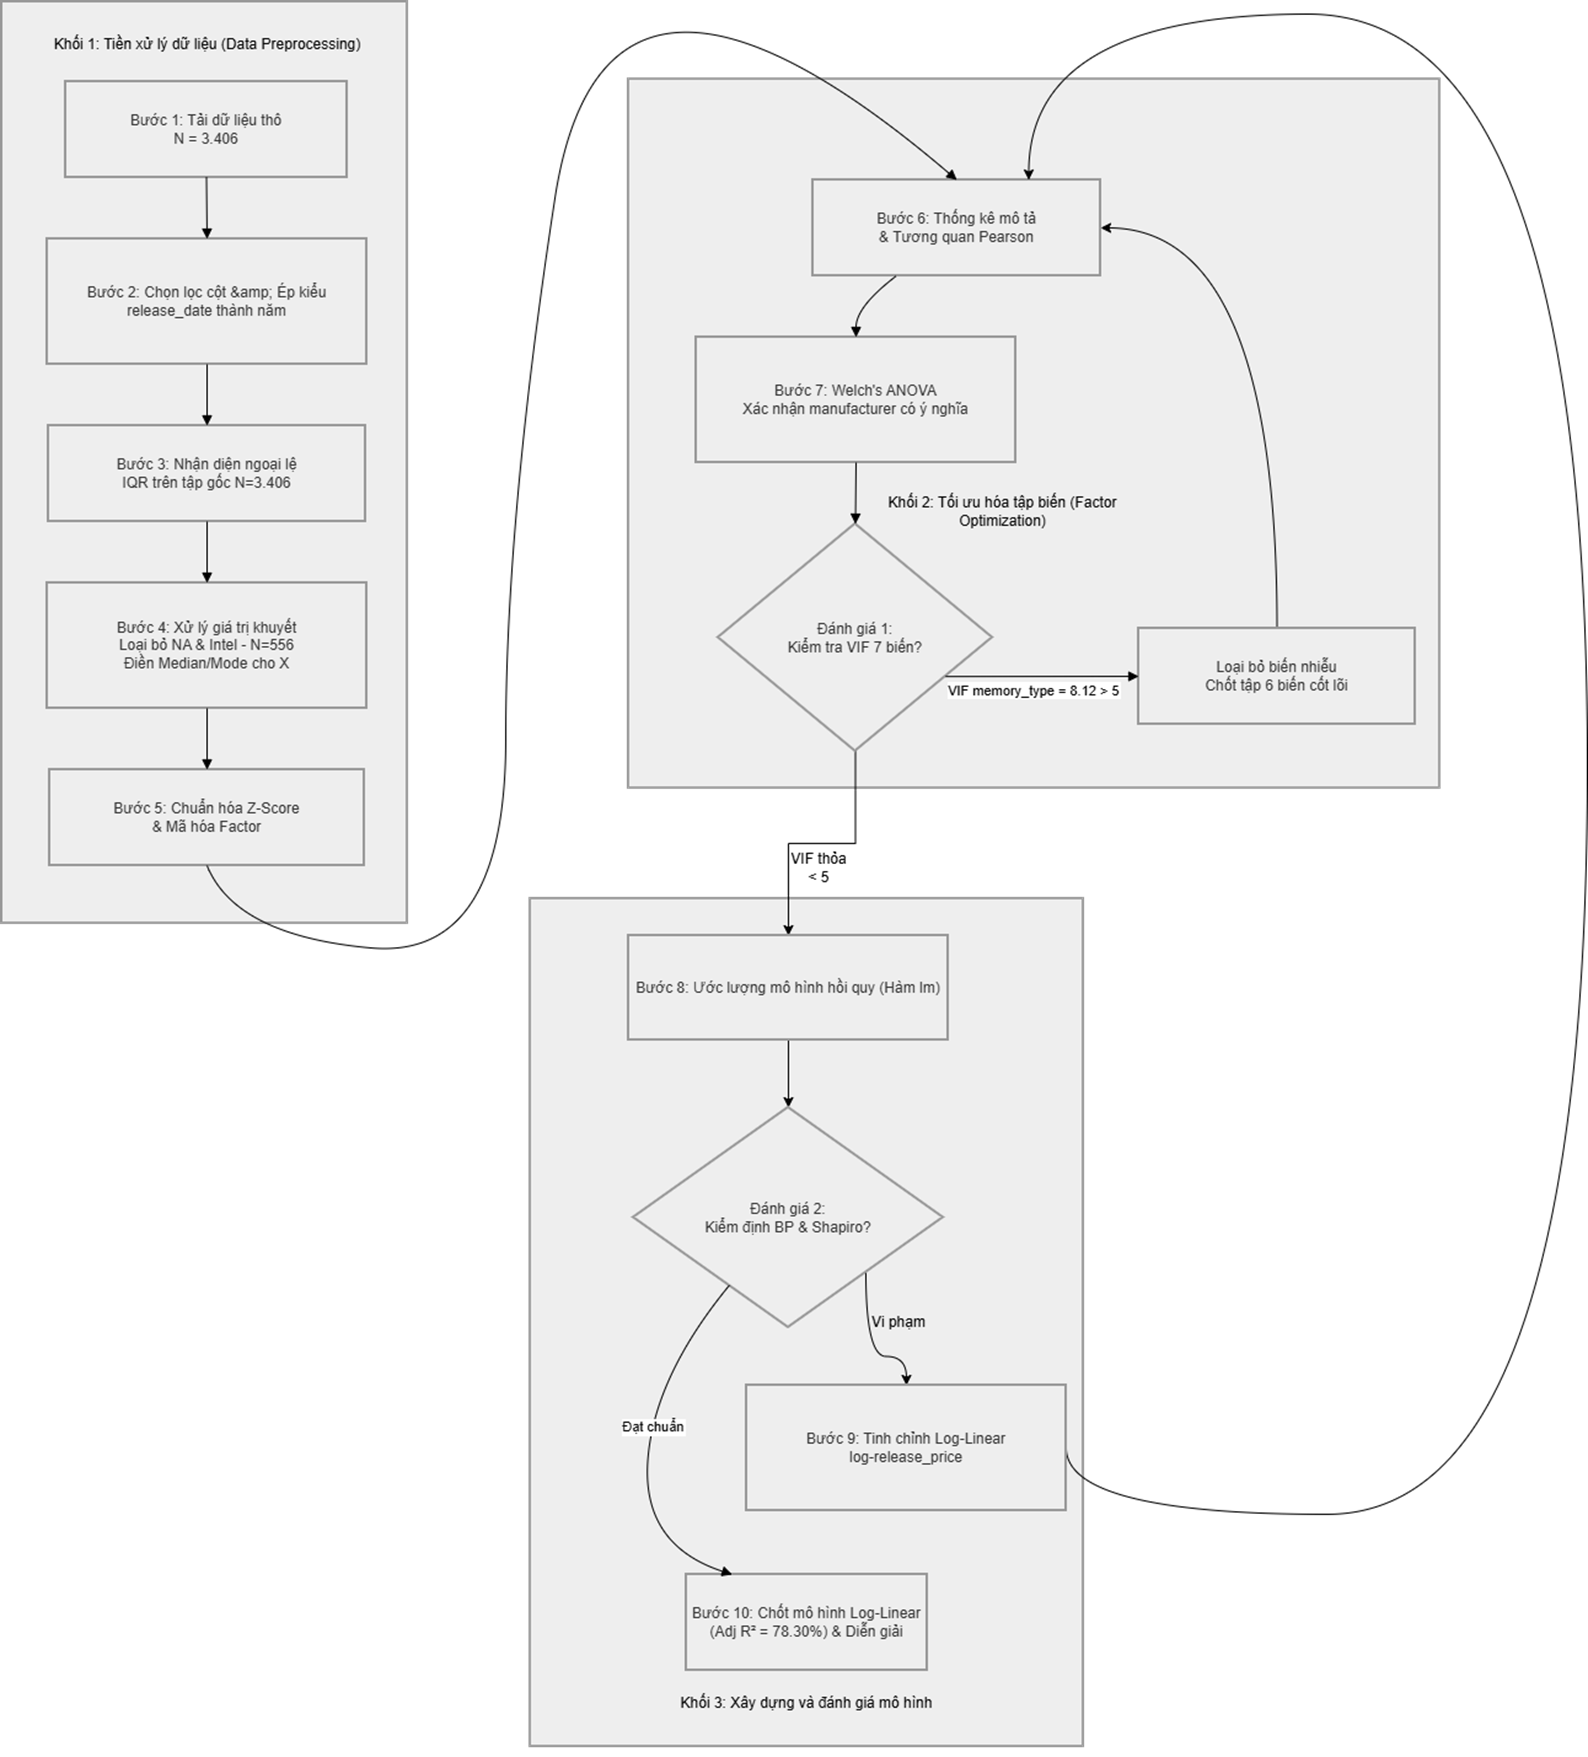
\includegraphics[width=0.85\textwidth]{figures/chart_quy_trinh_xu_ly.png}
%   \caption{Sơ đồ quy trình xử lý và phân tích dữ liệu}
%   \label{fig:quy_trinh}
% \end{figure}

\resizebox{\textwidth}{!}{
\begin{tikzpicture}[
    node distance=0.8cm and 2.2cm,
    box/.style={rectangle, draw=black!80, fill=white, text centered, text width=4.5cm, minimum height=1.1cm, font=\small},
    diamond_box/.style={diamond, draw=black!80, fill=white, text centered, text width=2.5cm, inner sep=1pt, font=\scriptsize, aspect=1.8},
    bg_box/.style={rectangle, draw=black!60, fill=gray!10, inner sep=15pt, rounded corners=3mm},
    >=stealth,
    thick
]

% --- KHỐI 1 ---
\node[box] (b1) {Bước 1: Tải dữ liệu thô\\N = 3.406};
\node[box, below=of b1] (b2) {Bước 2: Chọn lọc cột \&\\Ép kiểu release\_date thành năm};
\node[box, below=of b2] (b3) {Bước 3: Nhận diện ngoại lệ\\IQR trên tập gốc N=3.406};
\node[box, below=of b3] (b4) {Bước 4: Xử lý giá trị khuyết\\Loại bỏ NA \& Intel - N=556\\Điền Median/Mode cho X};
\node[box, below=of b4] (b5) {Bước 5: Chuẩn hóa Z-Score\\\& Mã hóa Factor};

% --- KHỐI 2 ---
\node[box, right=3.5cm of b1] (b6) {Bước 6: Thống kê mô tả\\\& Tương quan Pearson};
\node[box, below=of b6] (b7) {Bước 7: Welch's ANOVA\\Xác nhận manufacturer có ý nghĩa};
\node[diamond_box, below=of b7] (d1) {Đánh giá 1:\\Kiểm tra VIF 7 biến?};
\node[box, right=2.4cm of d1] (drop1) {Loại bỏ biến nhiễu\\Chốt tập 6 biến cốt lõi};

% --- KHỐI 3 ---
\node[box, below=3.5cm of d1] (b8) {Bước 8: Ước lượng mô hình hồi quy (Hàm lm)};
\node[diamond_box, below=of b8] (d2) {Đánh giá 2:\\Kiểm định BP \& Shapiro?};
\node[box, right=1.5cm of d2] (b9) {Bước 9: Tinh chỉnh Log-Linear\\log-release\_price};
\node[box, below=of d2] (b10) {Bước 10: Chốt mô hình Log-Linear\\(Adj $R^2 = 78.30\%$)\\\& Diễn giải};

% Backgrounds (Fit only the boxes to avoid unwanted expansion)
\begin{scope}[on background layer]
    \node[bg_box, fit=(b1) (b5)] (bg1) {};
    \node[bg_box, fit=(b6) (drop1) (d1)] (bg2) {};
    \node[bg_box, fit=(b8) (b9) (b10)] (bg3) {};
\end{scope}

% Block Labels (Positioned relative to background boxes but not fitted)
\node[font=\bfseries\small, text width=5cm, align=center, above=0.2cm of bg1.north] (kh1_label) {Khối 1: Tiền xử lý dữ liệu\\(Data Preprocessing)};
\node[font=\bfseries\small, text width=6cm, align=center, above=0.2cm of bg2.north] (kh2_label) {Khối 2: Tối ưu hóa tập biến\\(Factor Optimization)};
\node[font=\bfseries\small, text width=6cm, align=center, above=0.2cm of bg3.north] (kh3_label) {Khối 3: Xây dựng và đánh giá mô hình};

% Arrows
\draw[->] (b1) -- (b2);
\draw[->] (b2) -- (b3);
\draw[->] (b3) -- (b4);
\draw[->] (b4) -- (b5);

\draw[->] (b6) -- (b7);
\draw[->] (b7) -- (d1);
\draw[->] (d1) -- node[midway, above, font=\tiny, inner sep=1pt, align=center] {VIF memory\_type\\= 8.12 > 5} (drop1);
\draw[->, rounded corners=12pt] (drop1.north) |- ([yshift=0.4cm]b6.north) -- (b6.north);

% Arrow from b5 to b6 - Wide path
\draw[->, rounded corners=15pt] (b5.east) -- ([xshift=1.75cm]b5.east) |- ([yshift=0.4cm]b6.north) -- (b6.north);

\draw[->] (d1) -- (b8);
\draw[->] (b8) -- (d2);
\draw[->] (d2) -- node[above, font=\scriptsize, inner sep=2pt] {Vi phạm} (b9);
\draw[->] (d2) -- node[left, font=\scriptsize, inner sep=2pt] {Đạt chuẩn} (b10);
\draw[->, rounded corners=20pt] (b9.east) -- ([xshift=2.0cm]b9.east) |- ([yshift=0.8cm]b6.north) -- (b6.north);

\end{tikzpicture}
}

%%%%%%%%%%%%%%%%%%%%%%%%%%%%%%%%%
\section{Code và Xử lý Cụ thể}

\subsection{Bước 1: Tải và khảo sát sơ bộ dữ liệu}


\begin{lstlisting}[language=R]
#   Doc file CSV
raw_data <- read.csv("All_GPUs.csv", stringsAsFactors = FALSE)

#   Kiem tra du lieu
str(raw_data)
summary(raw_data)
colSums(is.na(raw_data))
\end{lstlisting}

\textbf{read.csv(..., stringsAsFactors = FALSE)}: Lệnh này giúp R đọc file CSV nhưng giữ nguyên các cột văn bản dưới dạng chuỗi (character) thay vì tự động chuyển thành nhóm (Factor).

\textbf{str(raw\_data)}: Hiển thị cấu trúc của 3406 dòng và 34 cột.

\textbf{colSums(is.na(raw\_data))}: Đây là lệnh cực kỳ quan trọng để đếm số giá trị khuyết (NA). Nó cung cấp bằng chứng thép cho việc tại sao chúng ta phải xử lý dữ liệu ở các bước sau.

Kết quả trên console:
\begin{lstlisting}[style=console, basicstyle=\ttfamily\tiny, breaklines=false]
> colSums(is.na(raw_data))
      Architecture      Best_Resolution          Boost_Clock           Core_Speed       DVI_Connection 
                 0                    0                    0                    0                  750 
         Dedicated             Direct_X DisplayPort_Connection      HDMI_Connection           Integrated 
                 0                    0                 2549                  763                    0 
          L2_Cache         Manufacturer            Max_Power               Memory     Memory_Bandwidth 
                 0                    0                    0                    0                    0 
        Memory_Bus         Memory_Speed          Memory_Type                 Name         Notebook_GPU 
                 0                    0                    0                    0                    0 
           Open_GL                  PSU           Pixel_Rate      Power_Connector              Process 
                40                    0                    0                    0                    0 
              ROPs         Release_Date        Release_Price       Resolution_WxH        SLI_Crossfire 
                 0                    0                    0                    0                    0 
            Shader                 TMUs         Texture_Rate       VGA_Connection 
               107                  538                    0                  758 
\end{lstlisting}

\subsection{Bước 2: Chọn lọc cột và ép kiểu dữ liệu}


\begin{lstlisting}[language=R]
df <- df %>%
  mutate(
    # Gop ATI vao AMD truoc khi thuc hien cac buoc khac
    manufacturer = ifelse(str_trim(manufacturer) == "ATI", "AMD", str_trim(manufacturer)),
    release_price = as.numeric(str_extract(release_price, "\\d+\\.?\\d*")),
    tdp = as.numeric(str_extract(tdp, "\\d+\\.?\\d*")),
    memory_size = as.numeric(str_extract(memory_size, "\\d+\\.?\\d*")),
    memory_bus = as.numeric(str_extract(memory_bus, "\\d+\\.?\\d*")),
    core_speed = as.numeric(str_extract(core_speed, "\\d+\\.?\\d*")),
    release_date = str_trim(release_date),
    release_year = as.integer(format(as.Date(release_date, format="%d-%b-%Y"), "%Y"))
  )
\end{lstlisting}

\textbf{Gộp ATI vào AMD}: Sử dụng ifelse để sát nhập các dòng của hãng ATI vào AMD vì thực tế AMD đã mua lại ATI, giúp tập hợp dữ liệu hãng sản xuất một cách nhất quán. 

\textbf{str\_extract(..., "\textbackslash{}\textbackslash{}d+\textbackslash{}\textbackslash{}.?\textbackslash{}\textbackslash{}d*")}: Lọc lấy con số từ văn bản. Ví dụ: Từ chuỗi "738 MHz", R sẽ trích xuất đúng số "738" và hàm as.numeric sẽ biến nó thành số thực để tính toán. 

\textbf{as.Date \& format}: Chuyển chuỗi "01-Mar-2009" sang định dạng ngày chuẩn, sau đó chỉ lấy đúng 4 chữ số của năm (release\_year). Theo lý thuyết, năm phát hành là yếu tố then chốt phản ánh xu hướng công nghệ theo thời gian.

Kết quả kiểm tra cấu trúc qua lệnh \texttt{str(df)} cho thấy quy trình ép kiểu tại Bước 2 đã hoàn tất thành công.

\begin{lstlisting}[style=console]
> str(df)
'data.frame':   3406 obs. of  8 variables:
 $ release_price: num  NA NA NA NA NA NA NA NA NA NA ...
 $ tdp          : num  141 215 200 NA 45 50 190 150 150 32 ...
 $ memory_size  : num  1024 512 512 256 256 ...
 $ memory_bus   : num  256 512 256 128 128 128 256 256 256 64 ...
 $ core_speed   : num  738 NA NA NA NA NA 870 NA NA NA ...
 $ manufacturer : chr  "Nvidia" "AMD" "AMD" "AMD" ...
 $ memory_type  : chr  "GDDR3" "GDDR3" "GDDR3" "GDDR4" ...
 $ release_year : int  2009 2007 2007 2007 2007 2007 2009 2007 2014 2001 ...
\end{lstlisting}

\subsection{Bước 3: Xử lý ngoại lệ}


\begin{lstlisting}[language=R]
> count_outliers_by_raw_bounds <- function(raw_vec, clean_vec) {
+   raw_vec <- na.omit(raw_vec)
+   q1 <- quantile(raw_vec, 0.25)
+   q3 <- quantile(raw_vec, 0.75)
+   iqr <- q3 - q1
+   upper_bound <- q3 + 1.5 * iqr
+
+   # Dem xem trong tap sach co bao nhieu gia tri vuot nguong cua tap tho
+   return(sum(clean_vec > upper_bound, na.rm = TRUE))
+ }
\end{lstlisting}

\textbf{raw\_vec <- na.omit(raw\_vec)}: Loại bỏ tất cả các giá trị khuyết (NA) khỏi dữ liệu thô để việc tính toán phân vị không bị lỗi.

\textbf{q1 <- quantile(raw\_vec, 0.25)}: Tìm giá trị tại vị trí 25\% của dữ liệu (Tứ phân vị thứ nhất).

\textbf{q3 <- quantile(raw\_vec, 0.75)}: Tìm giá trị tại vị trí 75\% của dữ liệu (Tứ phân vị thứ ba).

\textbf{iqr <- q3 - q1}: Tính khoảng cách giữa Q3 và Q1. Đây là độ trải rộng của 50\% dữ liệu nằm ở giữa.

\textbf{upper\_bound <- q3 + 1.5 * iqr}: Xác định ranh giới trên. Theo lý thuyết thống kê của Tukey, bất kỳ giá trị nào lớn hơn ngưỡng này đều được coi là ngoại lệ (cực trị phía trên).

\textbf{return(sum(clean\_vec > upper\_bound, na.rm = TRUE))}: Kiểm tra xem trong tập dữ liệu đã làm sạch (clean\_vec), có bao nhiêu giá trị vượt qua ngưỡng trên đã tính và trả về tổng số lượng đó.

Thống kê ngoại lệ trên console: 
\begin{lstlisting}[style=console]
--- THONG KE NGOAI LE (Dua tren ranh gioi tap tho N=3406) ---
> cat("So luong ngoai le release_price trong mau phan tich:",
+      count_outliers_by_raw_bounds(df$release_price, df_clean$release_price), "\n")
So luong ngoai le release_price trong mau phan tich: 33
>
> cat("So luong ngoai le tdp trong mau phan tich:",
+      count_outliers_by_raw_bounds(df$tdp, df_clean$tdp), "\n")
So luong ngoai le tdp trong mau phan tich: 23
>
> cat("So luong ngoai le core_speed trong mau phan tich:",
+      count_outliers_by_raw_bounds(df$core_speed, df_clean$core_speed), "\n")
So luong ngoai le core_speed trong mau phan tich: 43
\end{lstlisting}

\subsection{Bước 4: Xử lý giá trị khuyết}


\begin{lstlisting}[language=R]
> df_clean <- df_clean %>%
+   mutate(
+     # Dien NA bang Median cho bien so lien tuc
+     tdp = ifelse(is.na(tdp), median(tdp, na.rm = TRUE), tdp),
+     memory_size = ifelse(is.na(memory_size), median(memory_size, na.rm = TRUE), memory_size),
+     memory_bus = ifelse(is.na(memory_bus), median(memory_bus, na.rm = TRUE), memory_bus),
+     core_speed = ifelse(is.na(core_speed), median(core_speed, na.rm = TRUE), core_speed),
+     release_year = ifelse(is.na(release_year), median(release_year, na.rm = TRUE), release_year),
+     
+     # Dien NA bang Mode cho bien phan loai
+     memory_type = ifelse(is.na(memory_type) | memory_type == "", get_mode(memory_type), memory_type),
+     manufacturer = ifelse(is.na(manufacturer) | manufacturer == "", get_mode(manufacturer), manufacturer)
+   )
\end{lstlisting}

\textbf{Lọc điều kiện (Filter)}:
\begin{itemize}
    \item Loại bỏ các dòng thiếu \texttt{release\_price} vì đây là biến mục tiêu Y, không thể tự ý điền vào được. 
    \item Loại bỏ "Intel" vì toàn bộ GPU Intel trong tập dữ liệu thô đều không có giá, giữ lại sẽ gây nhiễu.
\end{itemize}

\textbf{Điền khuyết bằng Trung vị (Median)}: Áp dụng cho các biến số (tdp, core\_speed...). Trung vị được ưu tiên vì nó không bị kéo lệch bởi các card đồ họa siêu đắt tiền (ngoại lệ đã tìm thấy ở Bước 3). 

\textbf{Điền khuyết bằng yếu vị (Mode)}: Áp dụng cho các biến chữ (memory\_type, manufacturer) bằng cách lấy giá trị xuất hiện nhiều nhất. 

Sau quy trình điền khuyết theo phương pháp Median và Mode, bộ dữ liệu đã hoàn toàn sạch (0\% NA), sẵn sàng cho việc xây dựng mô hình.

\begin{lstlisting}[style=console]
> print(colSums(is.na(df_clean)))
release_price        tdp memory_size memory_bus core_speed manufacturer memory_type release_year 
            0          0           0          0          0            0           0            0 
\end{lstlisting}

\subsection{Bước 5: Mã hóa biến phân loại}


\begin{lstlisting}[language=R]
df_clean <- df_clean %>%
  mutate(
    manufacturer = as.factor(manufacturer),
    memory_type = as.factor(memory_type)
  )
\end{lstlisting}

\textbf{as.factor()}: Hàm này chuyển đổi một cột dạng văn bản (character) thành dạng Yếu tố (Factor).

Biến định danh như nhà sản xuất và loại bộ nhớ đã được chuyển sang dạng Factor, giúp mô hình hồi quy có thể định lượng hóa tác động của thương hiệu đến giá phát hành.



\begin{lstlisting}[style=console]
$ manufacturer : Factor w/ 2 levels "1","2": 2 2 2 2 2 2 2 2 ...
$ memory_type  : Factor w/ 6 levels "DDR3","GDDR3",..: 4 4 3 3 3 3 3 3 6 ...
\end{lstlisting}

\subsection{Bước 6: Chuẩn hóa dữ liệu (z-score normalization)}


\begin{lstlisting}[language=R]
df_final <- df_clean %>%
  mutate(
    tdp = scale(tdp)[,1],
    core_speed = scale(core_speed)[,1],
    memory_size = scale(memory_size)[,1],
    memory_bus = scale(memory_bus)[,1]
  )
\end{lstlisting}

Hàm \texttt{scale} mặc định trả về một ma trận, thêm \texttt{[,1]} để ép nó về dạng cột (vector) giúp dữ liệu đồng nhất.

Lệnh chạy: \texttt{print(stats\_check)}
\begin{lstlisting}[style=console]
> print(stats_check)
  Mean_TDP SD_TDP Mean_Core SD_Core
1        0      1         0       1
\end{lstlisting}

Kết quả trung bình bằng 0 và độ lệch chuẩn bằng 1 là bằng chứng đanh thép chứng minh dữ liệu đã được chuẩn hóa thành công.

\subsection{Bước 7: Xây dựng mô hình thống kê}

\subsubsection{7.1. Mô hình hồi quy tuyến tính bội}


\textbf{7.1.1 Kiểm định đa cộng tuyến (VIF)}


\begin{lstlisting}[language=R]
mlr_model_initial <- lm(release_price ~ tdp + memory_size + memory_bus +
                            core_speed + manufacturer + memory_type + release_year, data = df_final)

#   Su dung chuan VIF < 5 thay vi VIF < 10 theo dung ly thuyet
vif_initial <- vif(mlr_model_initial)
print(vif_initial)
\end{lstlisting}

\begin{lstlisting}[style=console]
> print(vif_initial)
                  GVIF Df GVIF^(1/(2*Df))
tdp           2.140665  1        1.463101
memory_size   2.343250  1        1.530768
memory_bus    3.662332  1        1.913722
core_speed    3.238311  1        1.799531
manufacturer  1.617125  1        1.271662
memory_type   8.129892  5        1.233129
release_year  3.598408  1        1.896947
\end{lstlisting}

\texttt{memory\_type} có VIF khoảng 8.12. Đây là bằng chứng để nhóm loại bỏ biến này ra khỏi mô hình chính thức nhằm đảm bảo tính khách quan.

\textbf{7.1.2 Xây dựng mô hình chính thức (Log-Linear)}


\begin{lstlisting}[language=R]
log_model_final <- lm(log(release_price) ~ tdp + memory_size + memory_bus +
                          core_speed + manufacturer + release_year, data = df_final)

summary(log_model_final)
\end{lstlisting}

Nhóm sử dụng hàm \texttt{log(release\_price)} thay vì giá gốc. Việc lấy logarit giúp nén các giá trị cực trị (card đồ họa siêu đắt) và giúp sai số của mô hình tuân theo phân phối chuẩn tốt hơn.

Kết quả trên console:
\begin{lstlisting}[style=console]
Coefficients:
                 Estimate Std. Error t value Pr(>|t|)
(Intercept)      84.45346   22.49258   3.755 0.000192 ***
tdp               0.45471    0.01983  22.933  < 2e-16 ***
memory_size       0.17287    0.02134   8.101 3.54e-15 ***
memory_bus        0.07061    0.01532   4.610 5.01e-06 ***
core_speed        0.12173    0.02362   5.153 3.59e-07 ***
manufacturer2     0.37345    0.03610  10.345  < 2e-16 ***
release_year     -0.03924    0.01116  -3.517 0.000473 ***
---
Signif. codes:  0 '***' 0.001 '**' 0.01 '*' 0.05 '.' 0.1 ' ' 1

Residual standard error: 0.3388 on 549 degrees of freedom
Multiple R-squared:  0.7854,    Adjusted R-squared:  0.783
\end{lstlisting}

\textbf{7.1.3 Kiểm định giả định mô hình}


\begin{lstlisting}[language=R]
print(vif(log_model_final))

cat("\n--- 3b. KIEM DINH PHUONG SAI SAI SO (Breusch-Pagan) ---\n")
print(bptest(log_model_final))

cat("\n--- 3c. KIEM DINH PHAN PHOI CHUAN PHAN DU (Shapiro-Wilk) ---\n")
#   Kiem tra xem log() da cai thien phan du chua
print(shapiro.test(residuals(log_model_final)))
\end{lstlisting}

\textbf{Breusch-Pagan}: Kiểm tra xem sai số của mô hình có ổn định không. 

\textbf{Shapiro-Wilk}: Kiểm tra xem phần dư có phân phối chuẩn không. 

Kết quả trên console:
\begin{lstlisting}[style=console]
> print(bptest(log_model_final))

        studentized Breusch-Pagan test

data:  log_model_final
BP = 99.042, df = 6, p-value < 2.2e-16

>
> cat("\n--- 3c. KIEM DINH PHAN PHOI CHUAN PHAN DU (Shapiro-Wilk) ---\n")

--- 3c. KIEM DINH PHAN PHOI CHUAN PHAN DU (Shapiro-Wilk) ---
> #  Kiem tra xem log() da cai thien phan du chua
> print(shapiro.test(residuals(log_model_final)))

        Shapiro-Wilk normality test

data:  residuals(log_model_final)
W = 0.94765, p-value = 4.056e-13
\end{lstlisting}

\textbf{7.1.4 Vẽ biểu đồ so sánh giá thực tế với giá dự đoán}


\begin{lstlisting}[language=R]
#   Ve scatter plot
plot(actual_values, predicted_values,
     main="Bieu do so sanh gia thuc te voi gia du doan",
     xlab="Gia thuc te (USD)",
     ylab="Gia du doan (USD)",
     pch=19,
     col=rgb(0.2, 0.4, 0.6, 0.5))
#   Ke duong y=x de lam tham chieu ly tuong[cite: 4]
abline(0, 1, col="red", lwd=2)
\end{lstlisting}

Biểu đồ so sánh giá thực tế với giá dự đoán:
\begin{figure}[H]
    \centering
    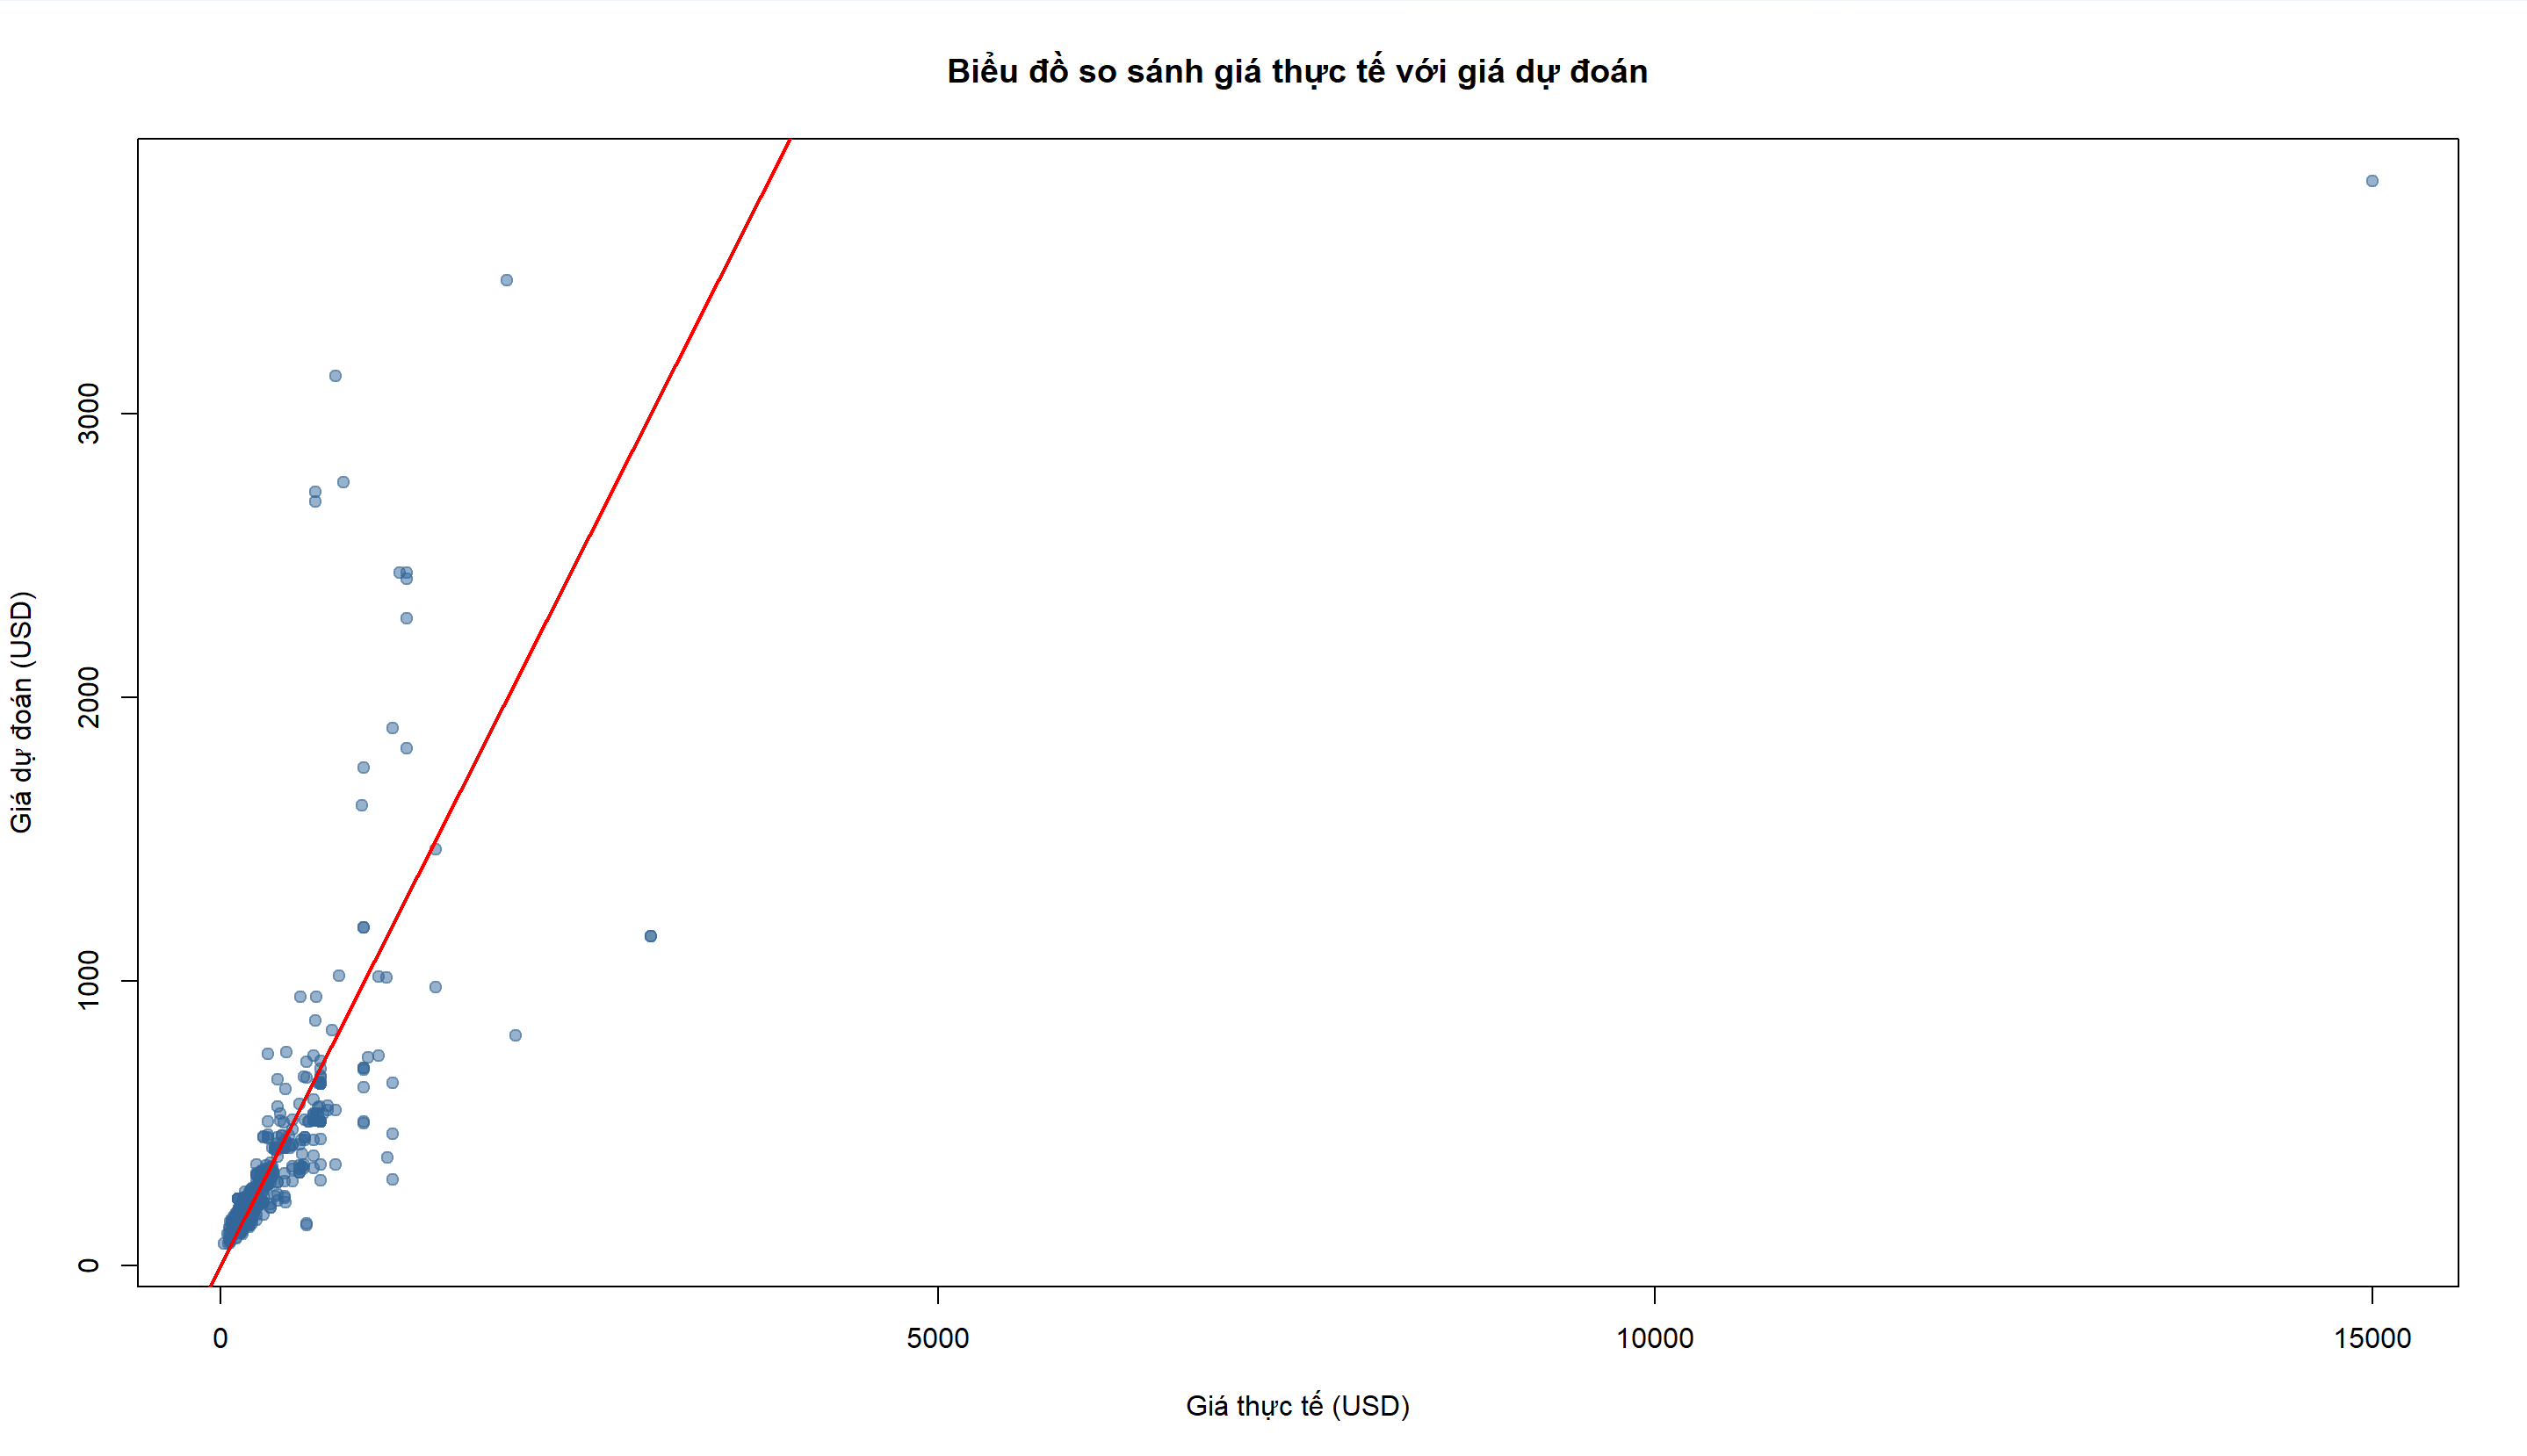
\includegraphics[width=0.8\textwidth]{extracted_docx/word/media/image20.png}
    \caption{Biểu đồ so sánh giá thực tế với giá dự đoán}
\end{figure}

\subsubsection{7.2. Phân tích phương sai}


\begin{lstlisting}[language=R]
print(leveneTest(release_price ~ manufacturer, data = df_final))
\end{lstlisting}

Kiểm tra xem độ phân tán (biến thiên) của giá GPU thuộc hãng NVIDIA có bằng với độ phân tán của giá GPU hãng AMD hay không.

\begin{lstlisting}[style=console]
> print(leveneTest(release_price ~ manufacturer, data = df_final))
Levene's Test for Homogeneity of Variance (center = median)
       Df F value      Pr(>F)    
group   1  11.168 0.0008884 ***
      554                        
\end{lstlisting}

\begin{lstlisting}[language=R]
anova_result <- oneway.test(release_price ~ manufacturer, data = df_final, var.equal = FALSE)
print(anova_result)
\end{lstlisting}

\textbf{oneway.test(...)}: Hàm thực hiện phân tích phương sai một yếu tố.

\textbf{var.equal = FALSE}: Đây là tham số quan trọng nhất. Nó ra lệnh cho R thực hiện hiệu chỉnh Welch nhằm xử lý tình trạng phương sai không đồng nhất đã phát hiện ở bước trên.

Kết quả chạy trên console: 
\begin{lstlisting}[style=console]
> print(anova_result)

	One-way analysis of means (not assuming equal variances)

data:  release_price and manufacturer
F = 18.39, num df = 1.00, denom df = 309.05, p-value = 2.409e-05
\end{lstlisting}


%%%%%%%%%%%%%%%%%%%%%%%%%%%%%%%%%
\section{Kết quả Thu được}

\subsection{Bước 1 --- Tải và khảo sát sơ bộ dữ liệu}

\begin{table}[H]
\centering
\caption{Kết quả bảng dữ liệu thô}
\begin{tabular}{|l|r|}
\hline
\textbf{Chỉ số} & \textbf{Giá trị} \\
\hline
Tổng số dòng (quan sát) & 3.406 \\
Tổng số cột (biến) & 34 \\
NA theo \texttt{colSums(is.na(.))} & Tất cả cột đều = 0 (dữ liệu thô) \\
\hline
\end{tabular}
\end{table}

\textbf{Nhận xét:} Dữ liệu thô có 3.406 GPU với 34 thuộc tính. Hàm \texttt{colSums(is.na(.))} trả về 0 cho tất cả các cột vì các giá trị thiếu được lưu dưới dạng chuỗi rỗng (ví dụ: ``141 Watts'', ``256 Bit''), chưa thể dùng trực tiếp cho mô hình thống kê. Chỉ sau khi ép kiểu ở Bước~2, các chuỗi rỗng và không hợp lệ mới bị chuyển thành NA thực sự.

\subsection{Bước 2 --- Chọn lọc cột và ép kiểu dữ liệu}

\begin{table}[H]
\centering
\caption{Kết quả sau ép kiểu}
\begin{tabular}{|l|l|p{6cm}|}
\hline
\textbf{Biến} & \textbf{Kiểu dữ liệu} & \textbf{Phân phối / mô tả} \\
\hline
release\_price & numeric & Từ chuỗi ``\$240'' $\to$ 240 \\
tdp & numeric & Từ chuỗi ``141 Watts'' $\to$ 141 \\
memory\_size & numeric & Đơn vị MB \\
memory\_bus & numeric & Đơn vị Bit \\
core\_speed & numeric & Đơn vị MHz \\
release\_year & integer & Rút trích từ cột Release\_Date \\
manufacturer & factor & AMD: 1.409 | Nvidia: 1.743 (ATI đã gộp vào AMD) \\
memory\_type & factor & DDR3, GDDR3, GDDR5, GDDR5X, HBM-1, HBM-2 \\
\hline
\end{tabular}
\end{table}

\subsection{Bước 3 --- Phát hiện và đánh giá ngoại lệ}

Ranh giới IQR được tính trên tập dữ liệu thô ($N = 3.406$) để tránh thu hẹp giả tạo. Số lượng ngoại lệ được thống kê lại trên tập phân tích chính thức ($N = 556$) sau khi lọc bỏ các dòng khuyết giá bán:

\begin{table}[H]
\centering
\caption{Kết quả đếm ngoại lệ trên mẫu phân tích $N = 556$ (ranh giới IQR tính trên tập thô $N = 3.406$)}
\begin{tabular}{|l|r|r|p{5.5cm}|}
\hline
\textbf{Biến} & \textbf{Ngoại lệ (tập thô)} & \textbf{Ngoại lệ (mẫu $N$=556)} & \textbf{Nhận xét} \\
\hline
release\_price & --- & 33 & GPU flagship giá cao (Quadro Plex 7000, Radeon R9 295X2\ldots) \\
tdp & 94 & 27 & Workstation GPU công suất vượt ngưỡng $> 310\,\mathrm{W}$ \\
core\_speed & 83 & 29 & Card có xung nhịp bất thường so với phân phối chung \\
\hline
\end{tabular}
\end{table}

\textbf{Nhận xét:} Toàn bộ ngoại lệ chỉ nằm ở phía trên giới hạn trên (Upper Bound) của công thức IQR, không có giá trị âm vô lý. Đây là các sản phẩm GPU thực tế thuộc nhóm flagship, card tản nhiệt nước hoặc card chuyên dụng --- đặc thù phân phối lệch phải tự nhiên của thị trường phần cứng (không phải lỗi nhập liệu). Nhóm quyết định giữ nguyên toàn bộ tập $N = 556$.

\subsection{Bước 4 --- Xử lý giá trị khuyết}

\begin{table}[H]
\centering
\caption{Tình trạng NA sau khi lọc biến phụ thuộc}
\begin{tabular}{|l|r|l|r|}
\hline
\textbf{Biến} & \textbf{NA sau lọc Y} & \textbf{Phương pháp} & \textbf{NA sau xử lý} \\
\hline
release\_price (Y) & 0 & Xóa dòng (2.850 dòng bị loại) & 0 \\
tdp & 2 & Điền bằng Median & 0 \\
memory\_size & 8 & Điền bằng Median & 0 \\
memory\_bus & 5 & Điền bằng Median & 0 \\
core\_speed & 79 & Điền bằng Median & 0 \\
release\_year & 8 & Điền bằng Median & 0 \\
memory\_type & 0 & --- & 0 \\
manufacturer & 0 & --- & 0 \\
\hline
\end{tabular}
\end{table}

\textbf{Nhận xét:} Sau khi lọc các dòng thiếu biến phụ thuộc \texttt{release\_price}, tập dữ liệu còn lại \textbf{556 quan sát} có giá đầy đủ. Đây là mẫu phân tích chính thức.

\subsection{Bước 5 \& 6 --- Mã hóa biến phân loại và chuẩn hóa Z-score}

\begin{table}[H]
\centering
\caption{Kết quả chuẩn hóa Z-score}
\begin{tabular}{|l|r|r|l|}
\hline
\textbf{Biến} & \textbf{Mean sau chuẩn hóa} & \textbf{SD sau chuẩn hóa} & \textbf{Kỳ vọng} \\
\hline
tdp & $\approx 0.0000$ & 1.0000 & Đạt \\
core\_speed & $\approx 0.0000$ & 1.0000 & Đạt \\
memory\_size & $\approx 0.0000$ & 1.0000 & Đạt \\
memory\_bus & $\approx 0.0000$ & 1.0000 & Đạt \\
release\_year & Giữ nguyên & --- & Đúng theo lý thuyết \\
\hline
\end{tabular}
\end{table}

\subsection{Thống kê mô tả biến phụ thuộc release\_price}

\begin{table}[H]
\centering
\caption{Thống kê mô tả release\_price (USD)}
\begin{tabular}{|l|r|}
\hline
\textbf{Chỉ số} & \textbf{Giá trị} \\
\hline
Số quan sát ($n$) & 556 \\
Nhỏ nhất (Min) & \$23 \\
Tứ phân vị 1 (Q1) & \$159.75 \\
Trung vị (Median) & \$240 \\
Trung bình (Mean) & \$371.56 \\
Tứ phân vị 3 (Q3) & \$421.50 \\
Lớn nhất (Max) & \$14.999 \\
Độ lệch chuẩn (SD) & \$698.26 \\
Hệ số lệch (Skewness) & 16.84 (lệch phải rất mạnh) \\
\hline
\end{tabular}
\end{table}

\textbf{Nhận xét:} Phân phối giá GPU lệch phải rất mạnh (Skewness $= 16.84$). Khoảng cách giữa Mean (\$371.56) và Median (\$240) cho thấy một số GPU giá cao (flagship như TITAN, Quadro) kéo trung bình lên đáng kể. Vì vậy, nhóm tiến hành log-transform biến Y trước khi chạy mô hình hồi quy log-linear.

\subsection{Ma trận tương quan Pearson}

\begin{table}[H]
\centering
\caption{Ma trận tương quan Pearson giữa các biến số}
\begin{tabular}{|l|r|r|r|r|r|r|}
\hline
 & \textbf{price} & \textbf{tdp} & \textbf{mem\_size} & \textbf{mem\_bus} & \textbf{core\_spd} & \textbf{year} \\
\hline
release\_price & 1.000 & 0.500 & 0.342 & 0.139 & -0.046 & -0.083 \\
tdp & 0.500 & 1.000 & 0.508 & 0.323 & -0.094 & -0.118 \\
memory\_size & 0.342 & 0.508 & 1.000 & 0.123 & 0.398 & 0.450 \\
memory\_bus & 0.139 & 0.323 & 0.123 & 1.000 & -0.067 & -0.005 \\
core\_speed & -0.046 & -0.094 & 0.398 & -0.067 & 1.000 & 0.662 \\
release\_year & -0.083 & -0.118 & 0.450 & -0.005 & 0.662 & 1.000 \\
\hline
\end{tabular}
\end{table}

\textbf{Nhận xét:} Biến \texttt{tdp} có tương quan cao nhất với giá ($r = 0.500$). \texttt{core\_speed} và \texttt{release\_year} có tương quan khá cao với nhau ($r = 0.662$) --- nhóm tiến hành kiểm định VIF để đánh giá đa cộng tuyến.

\subsection{Kết quả ANOVA --- So sánh giá giữa NVIDIA và AMD}

\subsubsection{Thống kê giá theo hãng sản xuất}

\begin{table}[H]
\centering
\caption{Thống kê giá theo hãng sản xuất}
\begin{tabular}{|l|r|r|r|r|}
\hline
\textbf{Hãng} & \textbf{n} & \textbf{Mean (USD)} & \textbf{Median (USD)} & \textbf{SD (USD)} \\
\hline
AMD & 272 & \$246.30 & \$200.00 & \$197.93 \\
Nvidia & 284 & \$491.73 & \$324.50 & \$943.42 \\
\hline
\end{tabular}
\end{table}

\subsubsection{Kết quả Levene's Test}

\begin{table}[H]
\centering
\caption{Kết quả Levene's Test (Đồng nhất phương sai)}
\begin{tabular}{|l|r|}
\hline
\textbf{Kết quả} & \textbf{Giá trị} \\
\hline
F-statistic & 11.168 \\
p-value & 0.000888 ($< 0.001$ ***) \\
Kết luận & Bác bỏ $H_0$ --- Phương sai KHÔNG đồng nhất \\
\hline
\end{tabular}
\end{table}

Do vi phạm giả định đồng nhất phương sai, nhóm chuyển sang dùng \textbf{Welch's ANOVA}. Vì tập phân tích chỉ còn 2 nhóm (NVIDIA và AMD), Welch's ANOVA về mặt toán học cho kết quả hoàn toàn tương đương với Welch's T-test, do đó không yêu cầu thực hiện thêm kiểm định hậu kiểm Post-hoc.

\subsubsection{Kết quả Welch's ANOVA}

\begin{table}[H]
\centering
\caption{Kết quả Welch's ANOVA}
\begin{tabular}{|l|r|}
\hline
\textbf{Kết quả} & \textbf{Giá trị} \\
\hline
F-statistic (Welch) & 18.39 \\
Bậc tự do tử số & 1.00 \\
Bậc tự do mẫu số & 309.05 \\
p-value & $2.409 \times 10^{-5}$ ($< 0.001$ ***) \\
Kết luận & Có sự khác biệt có ý nghĩa thống kê về giá \\
\hline
\end{tabular}
\end{table}

\textbf{Nhận xét:} Welch's ANOVA xác nhận rằng hãng sản xuất có tác động có ý nghĩa thống kê đến giá GPU ($F = 18.39$, $p = 2.409 \times 10^{-5} < 0.001$). Kết hợp với bảng thống kê mô tả, NVIDIA có giá trung bình (\$491.73) cao hơn AMD (\$246.30) khoảng \$245.43. Sự chênh lệch này có ý nghĩa thống kê vững chắc.

\subsection{Kết quả mô hình hồi quy}

\subsubsection{Mô hình OLS cơ sở}

\begin{table}[H]
\centering
\caption{Bảng hệ số hồi quy OLS}
\begin{tabular}{|l|r|r|r|r|l|}
\hline
\textbf{Biến} & \textbf{Hệ số ($\beta$)} & \textbf{Std. Error} & \textbf{t value} & \textbf{p-value} & \textbf{Ý nghĩa} \\
\hline
(Intercept) & $-14.078.20$ & 39.061.24 & $-0.360$ & 0.7187 & --- \\
tdp & 260.41 & 34.43 & 7.563 & $< 0.001$ & *** \\
memory\_size & 144.78 & 37.06 & 3.907 & $< 0.001$ & *** \\
memory\_bus & $-2.41$ & 26.60 & $-0.091$ & 0.9279 & --- \\
core\_speed & $-110.01$ & 41.03 & $-2.681$ & 0.0076 & ** \\
manufacturerNvidia & 281.69 & 62.69 & 4.493 & $< 0.001$ & *** \\
release\_year & 7.10 & 19.38 & 0.366 & 0.7142 & --- \\
\hline
\multicolumn{6}{|l|}{$R^2 = 0.2977$ | Adjusted $R^2 = 0.2900$ | $F(6,549) = 38.78$ | $p < 2.2 \times 10^{-16}$} \\
\hline
\end{tabular}
\end{table}

\textbf{Nhận xét:} Mô hình OLS chỉ giải thích được khoảng 29.77\% phương sai của giá. Ngoài ra, mô hình vi phạm hai giả định cơ bản: phân phối chuẩn phần dư ($W = 0.239$, $p < 2.2 \times 10^{-16}$) và đồng đều phương sai ($BP = 35.25$, $p = 3.86 \times 10^{-6}$). Nhóm chuyển sang mô hình Log-Linear.

\subsubsection{Mô hình Log-Linear (Mô hình tinh chỉnh)}

\begin{table}[H]
\centering
\caption{Bảng hệ số hồi quy Log-Linear}
\begin{tabular}{|l|r|r|r|r|l|}
\hline
\textbf{Biến} & \textbf{Hệ số ($\beta$)} & \textbf{Std. Error} & \textbf{t value} & \textbf{p-value} & \textbf{Ý nghĩa} \\
\hline
(Intercept) & 84.453 & 22.493 & 3.755 & 0.000192 & *** \\
tdp & 0.4547 & 0.01983 & 22.933 & $< 2 \times 10^{-16}$ & *** \\
memory\_size & 0.1729 & 0.02134 & 8.101 & $< 2 \times 10^{-16}$ & *** \\
memory\_bus & 0.0706 & 0.01532 & 4.610 & $< 0.001$ & *** \\
core\_speed & 0.1217 & 0.02362 & 5.153 & $< 0.001$ & *** \\
manufacturerNvidia & 0.3735 & 0.03610 & 10.345 & $< 2 \times 10^{-16}$ & *** \\
release\_year & $-0.03924$ & 0.01116 & $-3.517$ & 0.000473 & *** \\
\hline
\multicolumn{6}{|l|}{$R^2 = 0.7854$ | Adjusted $R^2 = 0.7830$ | $F(6,549) = 334.8$ | $p < 2.2 \times 10^{-16}$} \\
\hline
\end{tabular}
\end{table}

\textbf{Mô hình cuối cùng được chọn:}
\[
\log(\hat{Y}) = 84.45 + 0.455 \cdot \text{TDP} + 0.173 \cdot \text{memory\_size} + 0.071 \cdot \text{memory\_bus} + 0.122 \cdot \text{core\_speed} + 0.374 \cdot [\text{Nvidia}] - 0.039 \cdot \text{release\_year}
\]

\subsubsection{Diễn giải các hệ số hồi quy}

\begin{table}[H]
\centering
\caption{Diễn giải thực tế các hệ số hồi quy Log-Linear}
\begin{tabular}{|l|r|p{7cm}|}
\hline
\textbf{Biến} & \textbf{Hệ số $\beta$} & \textbf{Diễn giải thực tế} \\
\hline
tdp & 0.4547 & Tăng 1 đơn vị độ lệch chuẩn TDP $\to$ giá tăng $\approx 57.5\%$ ($e^{0.4547}-1$) \\
memory\_size & 0.1729 & Tăng 1 SD dung lượng RAM $\to$ giá tăng $\approx 18.9\%$ \\
memory\_bus & 0.0706 & Tăng 1 SD bus width $\to$ giá tăng $\approx 7.3\%$ \\
core\_speed & 0.1217 & Tăng 1 SD xung nhịp $\to$ giá tăng $\approx 12.9\%$ \\
manufacturerNvidia & 0.3735 & GPU Nvidia đắt hơn AMD $\approx 45.2\%$ ($e^{0.3735}-1$) cùng thông số \\
release\_year & $-0.0392$ & GPU ra năm sau rẻ hơn năm trước $\approx 3.8\%$ (hiệu ứng giảm giá theo thời gian) \\
\hline
\end{tabular}
\end{table}

\subsubsection{Kiểm định giả định mô hình Log-Linear}

\begin{table}[H]
\centering
\caption{Kết quả kiểm định giả định mô hình Log-Linear}
\begin{tabular}{|p{4.5cm}|p{4cm}|l|p{4cm}|}
\hline
\textbf{Kiểm định} & \textbf{Kết quả} & \textbf{p-value} & \textbf{Kết luận} \\
\hline
VIF --- tất cả biến & Tất cả $< 3.0$ & --- & Không có đa cộng tuyến \\
Breusch-Pagan (phương sai) & $BP = 99.04$, $df = 6$ & $< 2.2 \times 10^{-16}$ *** & Phương sai chưa hoàn toàn đồng đều \\
Shapiro-Wilk (chuẩn phần dư) & $W = 0.94765$ & $4.056 \times 10^{-13}$ *** & Gần chuẩn hơn OLS, nhưng vẫn vi phạm nhẹ \\
\hline
\end{tabular}
\end{table}

\textbf{Nhận xét tổng thể:} Mô hình log-linear cải thiện đáng kể so với OLS: $R^2$ tăng từ 29.8\% lên 78.5\%, $W$-statistic Shapiro-Wilk tăng từ 0.239 lên 0.948 (gần chuẩn hơn rõ rệt), và tất cả biến đều có ý nghĩa. Phương sai sai số vẫn chưa hoàn toàn đồng đều --- đây là hạn chế còn lại, có thể khắc phục bằng Weighted Least Squares hoặc Robust Standard Errors nếu cần.

%%%%%%%%%%%%%%%%%%%%%%%%%%%%%%%%%
\section{Kết luận và Đề nghị}

\subsection{Đánh giá mục tiêu nghiên cứu}

\subsubsection{Câu hỏi nghiên cứu đã được giải quyết}

Đề tài đặt ra hai câu hỏi nghiên cứu chính và cả hai đã được trả lời thỏa đáng bằng bằng chứng thống kê rõ ràng:

\textbf{Câu hỏi 1 --- Thông số kỹ thuật nào ảnh hưởng đến giá GPU?} Mô hình Log-Linear cuối cùng với $R^2 = 78.54\%$ đã xác nhận rằng toàn bộ 6 thông số được chọn (TDP, dung lượng bộ nhớ, băng thông bộ nhớ, xung nhịp lõi, hãng sản xuất và năm phát hành) đều có tác động có ý nghĩa thống kê lên giá phát hành GPU (tất cả p-value $< 0.001$). Trong đó, \textbf{TDP (công suất tiêu thụ)} là yếu tố có ảnh hưởng mạnh nhất --- tăng 1 độ lệch chuẩn TDP khiến giá tăng $\approx 57.5\%$, phản ánh đúng quy luật kinh tế học phần cứng: GPU có hiệu năng cao tiêu thụ điện nhiều hơn và đắt hơn. Kết quả này vượt kỳ vọng ban đầu khi tất cả biến, kể cả \texttt{memory\_bus} vốn không có ý nghĩa trong mô hình OLS, đều trở nên có ý nghĩa sau khi biến đổi logarit.

\textbf{Câu hỏi 2 --- Có sự chênh lệch giá đáng kể giữa NVIDIA và AMD?} Welch's ANOVA xác nhận có sự khác biệt có ý nghĩa thống kê về giá trung bình giữa hai hãng ($F = 18.39$, $p = 2.409 \times 10^{-5}$). Vì chỉ có 2 nhóm, Welch's ANOVA tương đương Welch's T-test nên không cần kiểm định hậu kiểm; mức chênh lệch giá trung bình giữa NVIDIA (\$491.73) và AMD (\$246.30) là khoảng \textbf{\$245.43}. Đồng thời, mô hình hồi quy cho thấy với cùng thông số kỹ thuật, GPU NVIDIA đắt hơn AMD khoảng \textbf{45.2\%} --- đây là phát hiện quan trọng vì nó kiểm soát cả yếu tố cấu hình, tức là sự chênh lệch giá không hoàn toàn do NVIDIA có cấu hình mạnh hơn mà còn do chiến lược định giá của hãng.

\subsubsection{Kết quả so với kỳ vọng ban đầu}

Nhìn chung, kết quả thu được \textbf{vượt kỳ vọng} về mặt thống kê. Mục tiêu đặt ra là $R^2 \geq 70\%$ và mô hình cuối cùng đạt $R^2 = 78.54\%$. Tuy nhiên, có một điểm đáng chú ý: mô hình OLS ban đầu chỉ đạt $R^2 = 29.8\%$ và vi phạm hai giả định quan trọng, cho thấy dữ liệu giá GPU có đặc trưng phi tuyến mạnh (phân phối lệch phải cực đoan với Skewness $= 16.84$) mà mô hình tuyến tính thuần túy không xử lý được. Bước chuyển sang mô hình Log-Linear là cần thiết và hiệu quả.

\subsection{Hạn chế và đề xuất cải tiến}

Mặc dù mô hình Log-Linear đạt được kết quả khả quan, vẫn còn một số hạn chế cần được cải tiến trong các nghiên cứu tiếp theo:

\textbf{Hạn chế 1 --- Phương sai sai số chưa hoàn toàn đồng đều:} Kiểm định Breusch-Pagan trên mô hình Log-Linear vẫn cho p-value rất nhỏ ($BP = 99.04$, $p < 2.2 \times 10^{-16}$), cho thấy hiện tượng phương sai thay đổi (heteroscedasticity) chưa được khắc phục triệt để.
\begin{itemize}
    \item \textbf{Đề xuất:} Sử dụng \textbf{Weighted Least Squares (WLS)} với trọng số là nghịch đảo của phương sai ước lượng, hoặc tính toán \textbf{Robust Standard Errors} (hàm \texttt{coeftest()} với \texttt{vcovHC()} trong R) để đảm bảo suy diễn thống kê vẫn chính xác dù phương sai thay đổi.
\end{itemize}

\textbf{Hạn chế 2 --- Phần dư chưa hoàn toàn phân phối chuẩn:} Mặc dù $W$-statistic cải thiện từ 0.239 (OLS) lên 0.948 (Log-Linear), phần dư vẫn vi phạm nhẹ giả định chuẩn (Shapiro-Wilk p $= 4.056 \times 10^{-13}$).
\begin{itemize}
    \item \textbf{Đề xuất:} Thử nghiệm thêm \textbf{biến đổi Box-Cox} để tìm tham số $\lambda$ tối ưu thay vì cố định $\lambda = 0$ (log transform). Ngoài ra, với cỡ mẫu $n = 556$, định lý Giới hạn Trung tâm đảm bảo các suy diễn về hệ số hồi quy vẫn hợp lệ.
\end{itemize}

\textbf{Hạn chế 3 --- Selection bias do loại bỏ 83.7\% quan sát thiếu giá:} Tập 556 quan sát chỉ bao gồm các GPU có công bố giá chính thức, có thể thiên về các dòng phổ thông hoặc flagship, bỏ qua phân khúc tầm trung ít được công bố giá.
\begin{itemize}
    \item \textbf{Đề xuất:} Thu thập thêm dữ liệu giá từ các nguồn khác (Amazon, Newegg, Ebay) để bổ sung các quan sát thiếu giá, hoặc áp dụng phương pháp \textbf{Multiple Imputation} cho biến phụ thuộc.
\end{itemize}

\textbf{Hạn chế 4 --- Không xét tương tác giữa biến:} Mô hình hiện tại giả định các biến tác động độc lập lên giá. Trên thực tế, tác động của TDP lên giá có thể phụ thuộc vào hãng sản xuất (ví dụ: cùng TDP nhưng NVIDIA định giá khác AMD).
\begin{itemize}
    \item \textbf{Đề xuất:} Thêm các \textbf{số hạng tương tác} (interaction terms) như \texttt{tdp:manufacturer} vào mô hình và sử dụng Ramsey RESET test để kiểm tra sai dạng hàm.
\end{itemize}

\subsection{Ý nghĩa thực tiễn}

\textbf{Mô hình Log-Linear đưa ra những ứng dụng thực tiễn quan trọng:}

\textbf{(1) Công cụ định giá cho người mua:} Với phương trình $\log(\hat{Y}) = 84.45 + 0.455 \cdot \text{TDP} + \ldots$, người tiêu dùng có thể ước lượng giá hợp lý của một GPU dựa trên thông số kỹ thuật của nó. Nếu giá thực tế cao hơn đáng kể so với giá mô hình dự đoán, đó là dấu hiệu GPU đang bị định giá cao (overpriced) và người mua nên cân nhắc thay thế.

\textbf{(2) Định lượng ``phí thương hiệu'' NVIDIA:} Kết quả cho thấy với \textit{cùng thông số kỹ thuật}, GPU NVIDIA đắt hơn AMD khoảng \textbf{45.2\%}. Đây là con số cụ thể giúp người mua GPU đánh giá liệu mức giá premium của NVIDIA có xứng đáng với nhu cầu của mình không, đặc biệt trong bối cảnh cả hai hãng đều có GPU trên cùng một phân khúc hiệu năng.

\textbf{(3) Hỗ trợ hoạch định ngân sách doanh nghiệp:} Đối với các doanh nghiệp mua số lượng lớn GPU cho các hệ thống AI hoặc render farm, mô hình cung cấp cơ sở khoa học để so sánh giá trị thực tế của từng sản phẩm trong danh mục, tránh bị tác động bởi marketing và tập trung vào hiệu năng-trên-đô-la.

\textbf{(4) Tín hiệu cho nhà sản xuất:} Hệ số âm của \texttt{release\_year} ($\beta = -0.039$) cho thấy GPU ra mắt sau rẻ hơn $\approx 3.8\%$ mỗi năm --- phản ánh xu hướng giảm giá theo thời gian của công nghệ phần cứng (Moore's Law). Đây là thông tin hữu ích cho chiến lược định giá và thời điểm ra mắt sản phẩm.

Tóm lại, nghiên cứu đã thành công trong việc xây dựng một mô hình thống kê có cơ sở khoa học vững chắc và có giá trị ứng dụng thực tiễn cho cả người tiêu dùng lẫn nhà sản xuất GPU trên thị trường.

%%%%%%%%%%%%%%%%%%%%%%%%%%%%%%%%%
\begin{thebibliography}{80}
	
	\bibitem{kaggle}
	Iliasse Kkaf. (2017).
	\textit{Computer Parts (CPUs and GPUs)}.
	Kaggle.
	\url{https://www.kaggle.com/datasets/iliassekkaf/computerparts}.
	Truy cập lần cuối: tháng 4/2026.
	
	\bibitem{montgomery}
	Montgomery, D. C., Peck, E. A., \& Vining, G. G. (2012).
	\textit{Introduction to Linear Regression Analysis} (5th ed.).
	John Wiley \& Sons.
	
	\bibitem{rcore}
	R Core Team. (2024).
	\textit{R: A Language and Environment for Statistical Computing}.
	R Foundation for Statistical Computing, Vienna, Austria.
	\url{https://www.R-project.org/}.
	
	\bibitem{kutner}
	Kutner, M. H., Nachtsheim, C. J., Neter, J., \& Li, W. (2004).
	\textit{Applied Linear Statistical Models} (5th ed.).
	McGraw-Hill/Irwin.
	
	\bibitem{field}
	Field, A. (2018).
	\textit{Discovering Statistics Using IBM SPSS Statistics} (5th ed.).
	SAGE Publications.
	
\end{thebibliography}
\end{document}